	\chapter{Introduction}
	% Disease background
	\section{Schizophrenia}
	\Gls{scz} is a devastating psychiatric disorder affecting approximately $0.3\sim0.7\%$ of the population  worldwide \citep{AmericanPsychiatricAssociation2013}.
	Generally, the typical age of onset of \gls{scz} is around late adolescent or late 20s in male and late 20s or early 30s in female \citep{Schultz2007}.
	
	
	\section{Schizophrenia}
	\Glng{scz} is a detrimental psychiatric disorder, affecting around $0.3\sim0.7\%$ of the population \citep{AmericanPsychiatricAssociation2013}.
	It is characterized by positive symptoms including delusions, hallucinations, disorganized speech and grossly disorganized behavior, and negative symptoms such as the diminished emotional expression \citep{AmericanPsychiatricAssociation2013} with a typical age of onset at late adolescent or late 20s in male and late 20s or early 30s in female \citep{Schultz2007}.
	
	\Glng{scz} not only impose long lasting health, social and financial burden to the patients, but also to their families \citep{Knapp2004}. 
	Moreover, patients with \glng{scz} have an increased tendency to suicide \citep{Saha2007}, leading to a higher mortality.
	Based on the \gls{who} report, \glng{scz} is one of the top 20 leading cause of \gls{yld} in 2012, ranking 16 among all possible causes (\cref{tab:whoYLD}), demonstrating the extent of impact from \glng{scz} to patients.
	\begin{table}[ht]
		\centering
		\caption[Top 20 leading cause of \glng{yld}]{Top 20 leading cause of \gls{yld} calculated by \gls{who} in year 2012.
			\Glng{scz} was considered as one of the top 20 leading cause of \gls{yld}\citep{Geneva2013}}
		\begin{tabular}{rrrrr}
			\toprule
			Rank  & Cause & \gls{yld} (000s) & \% \gls{yld} & \specialcell[b]{\gls{yld} per \\100k population}\\
			\midrule
			0     & All Causes & 740,545 & 100   & 10466 \\
			1     & Unipolar depressive disorders & 76,419 & 10.3  & 1080 \\
			2     & Back and neck pain & 53,855 & 7.3   & 761 \\
			3     & Iron-deficiency anaemia & 43,615 & 5.9   & 616 \\
			4     & Chronic obstructive pulmonary disease & 30,749 & 4.2   & 435 \\
			5     & Alcohol use disorders & 27,905 & 3.8   & 394 \\
			6     & Anxiety disorders & 27,549 & 3.7   & 389 \\
			7     & Diabetes mellitus & 22,492 & 3     & 318 \\
			8     & Other hearing loss & 22,076 & 3     & 312 \\
			9     & Falls & 20,409 & 2.8   & 288 \\
			10    & Migraine & 18,538 & 2.5   & 262 \\
			11    & Osteoarthritis & 18,096 & 2.4   & 256 \\
			12    & Skin diseases & 15,744 & 2.1   & 223 \\
			13    & Asthma & 14,134 & 1.9   & 200 \\
			14    & Road injury & 13,902 & 1.9   & 196 \\
			15    & Refractive errors & 13,498 & 1.8   & 191 \\
			16    & Schizophrenia & 13,408 & 1.8   & 189 \\
			17    & Bipolar disorder & 13,271 & 1.8   & 188 \\
			18    & Drug use disorders & 10,620 & 1.4   & 150 \\
			19    & Endocrine, blood, immune disorders & 10,495 & 1.4   & 148 \\
			20    & Gynecological diseases & 10,227 & 1.4   & 145 \\
			\bottomrule
		\end{tabular}%
		\label{tab:whoYLD}%
	\end{table}%
	
	Due to the severity of \glng{scz}, it has drawn much attention from the research community aiming to delineate the disease mechanics and be able to identify the risk factors and hopefully identify a cure to help improving the quality of life of the patients.
	Arguably, the most important first step to any \glng{scz} study is to have a robust and reliable disease diagnosis.
	
	\section{Diagnosis}
	% Describe early problems of diagnosis
	% Describe current method of diagnosis
	\Glng{scz} was first named ``Dementia Praecox'' by Dr. Emil Kraepelin and was later renamed as \glng{scz} by Dr. Eugen Bleuler \citep{Jablensky2010}.
	Early nosological entity for \glng{scz} such as that in \gls{dsm}-\rom{1} and \gls{dsm}-\rom{2} were vague and unreliable where the inter-rater agreement can be as low as 54\%. \citep{Tsuang2000,Harvey2012} 
	
	Later nosologies addressed these problem by introducing structural assessment and clear defined criteria. 
	With these improvements, the inter-rater agreement of \gls{dsm}-\rom{3} raised to $\sim 90\%$ \citep{Harvey2012}, suggesting the diagnosis were much more reliable.
	
	Currently \gls{dsm} is at its 5th edition \citep{AmericanPsychiatricAssociation2013}. 
	A patient will be diagnosed with \glng{scz} (F20.9) if they suffered from 2 or more of the following symptoms for a significant portion of time during a 1-month period: 
	\begin{enumerate*}[label=\arabic*\upshape)]
		\item delusion; \label{ls:delusion}
		\item hallucinations;\label{ls:hallucinations}
		\item disorganized speech;\label{ls:disorganizedSpeech}
		\item grossly disorganized or catatonic behaviour; and\label{ls:catatonicBehavior}
		\item negative symptoms such as diminished emotional expression,\label{ls:negativeSymptoms}
	\end{enumerate*}  where one of the symptom must be either (\ref{ls:delusion}, (\ref{ls:hallucinations} or (\ref{ls:disorganizedSpeech}.
	Signs of disturbance also need to persist for at least 6-month before the patient can be diagnosed with \glng{scz}.
	
	\section{Risk Factors of Schizophrenia}
	\sectionmark{Risk Factors}
	% Talk about brown's study, the increased risk of schizophrenia in the influenza epidemic
	% Talk about some other risk factors such as drug use etc
	Considerable effort has been made trying to identify possible risk factors of \glng{scz}. 
	It was first observed that there was an increased risk of \glng{scz} in individual who were fetuses during the 1957 influenza epidemic \citep{Mednick1958}. 
	Subsequently, other infectious agents such as HSV-2 and \textit{T.gondii} were also found to increase the risk of \glng{scz} if an individual's mother were infected during pregnancy.
	As different infectious agents all increase the risk of \glng{scz}, it leads to the hypothesis of \gls{mia} \citep{Brown2010}.
	It was hypothesized that instead of a particular infectious agents, it was the maternal immune response that disrupt the brain development in the offspring, thus leading to an elevated risk of \glng{scz}.

	As it is unethical to induce \gls{mia} in human, rodent models were utilize in order to test the effect of \gls{mia} to the fetal development. 
	It was found that prenatal infection and \gls{mia} can be modeled in the rodent; specifically the viral analogue \gls{polyic} precipitates a brain and behavioral phenotype in rodent offspring which mirrors that observed in schizophrenia and related neurodevelopmental conditions \citep{Li2009c,Meyer2009b,Li2010a}.
	One important property of \gls{polyic} is that it will only induce the \gls{mia} without infecting the fetuses. 
	Thus it provide strong evidence that it is the \gls{mia} instead of the infection that increases the risk of \glng{scz}.
	
	\citet{Smith2007} were able to show that a single injection of \gls{il6} to the pregnant mouse can induce \glng{scz}-like behaviour in the adult offspring. 
	What is most interesting was by eliminating the \gls{il6} from the maternal immune response using either genetic methods (\gls{il6} knock out) or with blocking antibodies, the behaviour deficits associated with \gls{mia} are not present in the adult offspring, suggesting that \gls{il6} is central to the process by which \gls{mia} causes long-term behavioral changes.
	
	Further studies of global gene expression patterns in \gls{mia}-exposed rodent fetal brains \citep{Oskvig2012,Garbett2012a} suggest that the post-pubertal onset of schizophrenic and other psychosis-related phenotypes might stem from attempts of the brain to counteract the environmental stress induced by \gls{mia} during its early development \citep{Garbett2012a}.
	Genes with neuroprotective function such as crystallins might also have additional roles in neuronal differentiation and axonal growth \citep{Garbett2012a}. 
	By over-expressing these genes to counteract the environmental stress, the balance between neurogenesis and differentiation in the embryonic brain be disrupted. 
	Based on these observations, \citet{Garbett2012a} propose that once the immune activation disappears, the normal brain development programme resumes with a time lag, resulting to in permanent changes in connectivity and neurochemistry that might ultimately leads to \glng{scz}-like behaviours.
	
	It was also demonstrated that \gls{mia} might leads to a complex pattern of age-dependent structural abnormalities in the mesoaccumbal and nigrostriatal dopamine systems\citep{Vuillermot2010}.
	Specifically, \gls{mia} induces an early abnormality in specific dopaminergic systems such as those in the striatum and midbrian region\citep{Vuillermot2010}.
	Based on these observations, \citet{Meyer2007a} hypothesize that inflammation in the fetal brain during early gestation not only can disrupt neurodavelopmental processes such as cell proliferation and differentiation, it also predispose the developing nervous system to additional failures in subsequent cell migration, target selection, and synapse maturation (\cref{fig:miaEffect}) \citep{Meyer2007a}.
	\begin{figure}
		\centering
		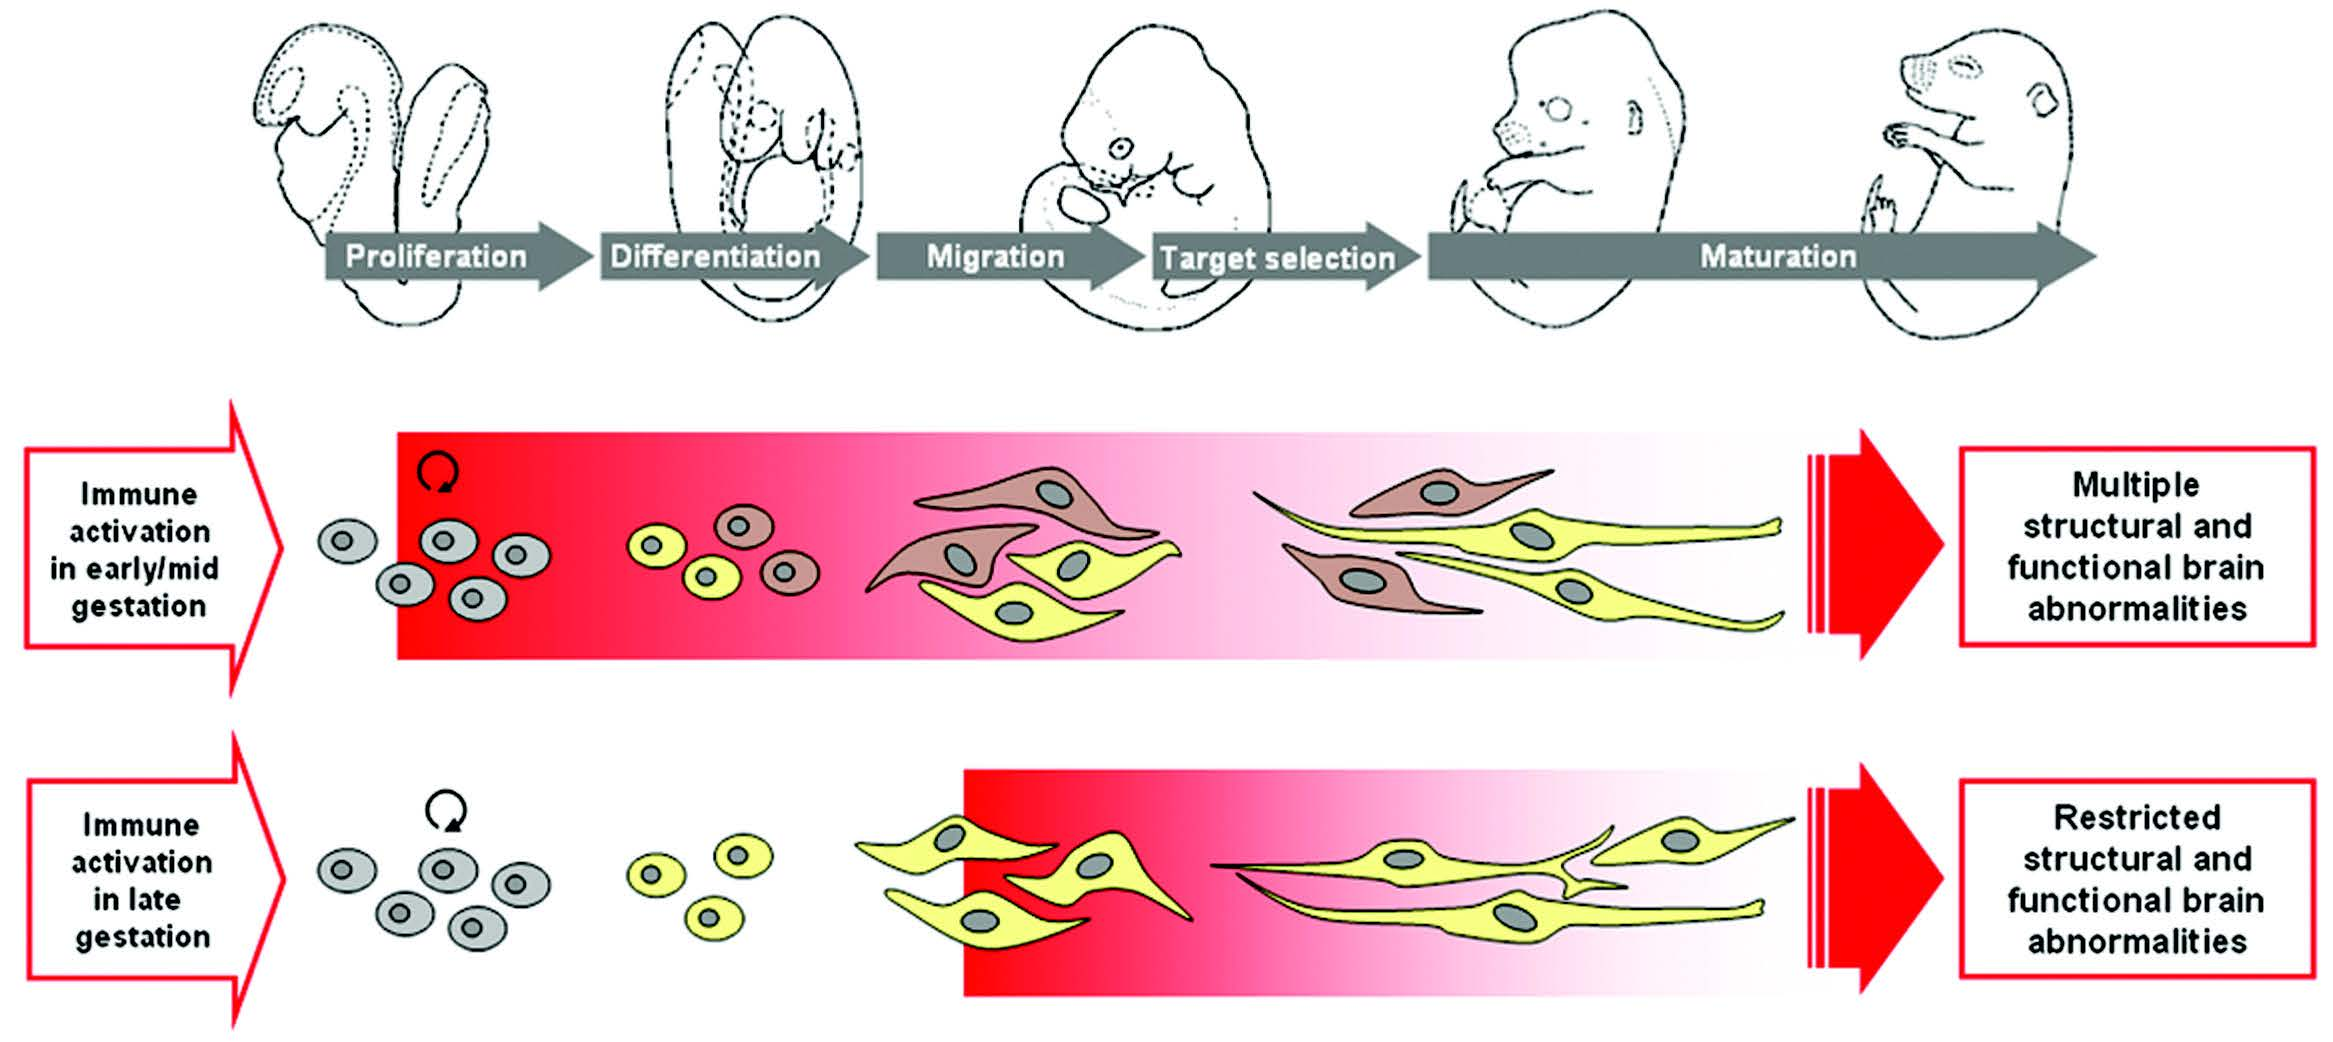
\includegraphics[width=\textwidth]{figure/mia_impact.jpg}
		\caption[Hypothesized model of the impact of prenatal immune challenge on fetal brain development]{Hypothesized model of the impact of prenatal immune challenge on fetal brain development.
			Maternal infection in early/mid pregnancy may affect early neurodevelopmental events in the fetal brain, thereby influencing the differentiation of neural precursor cells(grey) into particular neuronal phenotype(yellow or brown).
			This may predispose the developing fetal nervous system to additional failures leading to multiple structural and functional brain abnormalities in later life.
			Figure used with permission from Journal \citep{Meyer2007a}}
		\label{fig:miaEffect}
	\end{figure}
	
	In a separate study by \citet{Giovanoli2013}, mice were exposed to low dosage of \gls{polyic} during early gestation.
	Offspring born were then left undisturbed or exposed to unpredictable stress during peripubertal development.
	It was observed that offspring exposed to \gls{polyic} has an increased level of dopamine in the nucleus accumbens independent to whether if they were exposed to postnatal stress.
	Whereas serotonin (5-HT) were decreased in the medial prefrontal cortex when exposed to postnatal stress regardless of prenatal exposure.
	Only when the offspring were exposed to both \gls{polyic} and postnatal stress will they have an increased dopamine levels in the hippocampus or will sensorimotor gating and psychotomimetic drug sensitivity be affected \citep{Giovanoli2013}.
	\citet{Giovanoli2013} therefore suggest that the prenatal insult serves as a ``disease primer'' that increase offspring's vulnerability to subsequent insults.
	
	Another interesting observation in \citet{Giovanoli2013}'s study was that the combined immune activation and stress led to a 2.5 to 3 fold increase in hippocampal and prefrontal expression of markers characteristic of activated microglia.
	Considering that microglia is responsible for synaptic pruning during brain development \citep{Paolicelli2011}, perturbation of microglia in the fetal brain might also mediate \glng{scz}.
	Indeed, \citet{Onore2014} demonstrated that \gls{mia} has a prolonged effect on macrophages, leading to a shift towards to proinflammatory M1 phenotype.
	Immune dysfunction in the pathophysiology of \glng{scz} has long been speculated \citep{Muller2010a} and evidence shown that there was a strong influence of the pro- and anti-inflammation cytokines on the glutamatergic neurotransmission \citep{Muller2010a}, suggesting the immune system might played an important role in disease etiology of \gls{scz}.
	
	\begin{figure}
		\centering
		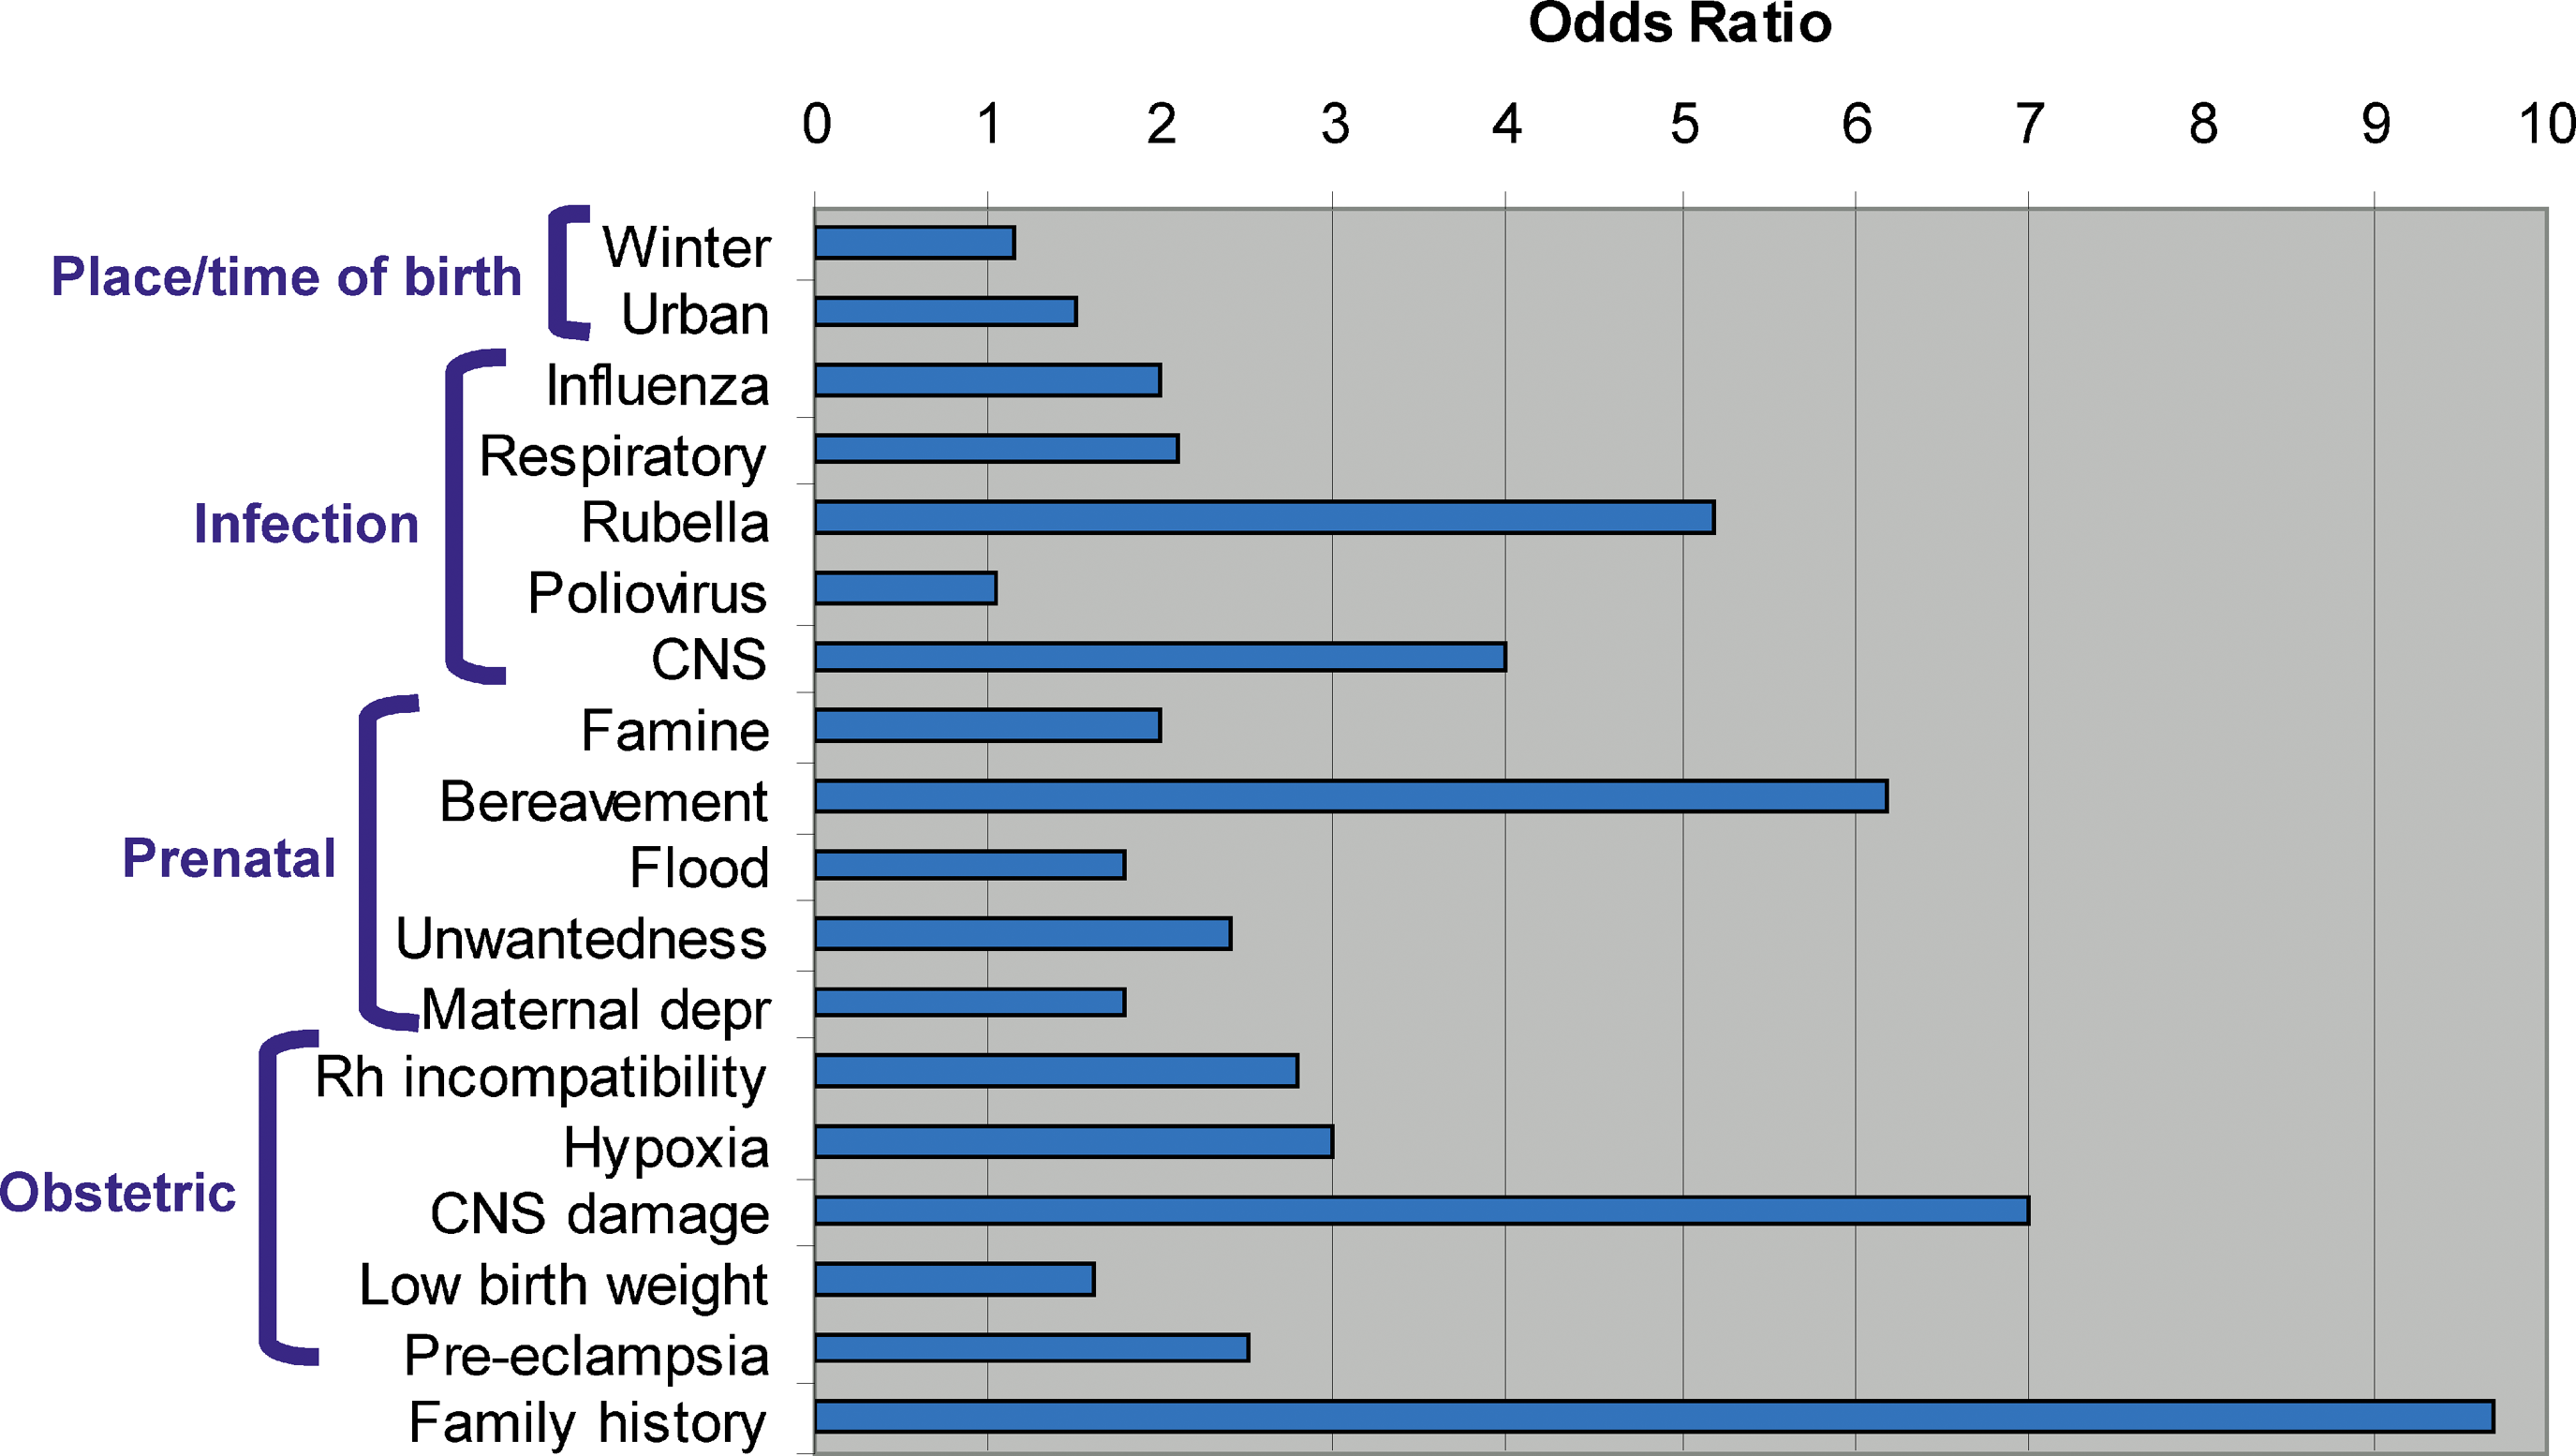
\includegraphics[width=\textwidth]{figure/risk_factors_of_schizophrenia.png}
		\caption[Risk factors of \glng{scz}]{Risk factors of \glng{scz}.
			It was observed that family history of \glng{scz} was the largest risk factors.
			Risk of \glng{scz} can be more than 9 times higher than the general population for individual with a family history of \glng{scz}}
		\label{fig:riskfactors}
	\end{figure}
	
	Together, these results supports the involvement of \gls{mia} in the development of \glng{scz}.
	It was even estimated that one third of all \glng{scz} cases could have been prevented shall all infection were prevented from the entire pregnant population \citep{Brown2010}.
	
	Similarly, tobacco consumption \citep{Kelly1999}, socio economic status and even the area of birth (e.g. urban vs suburb) were also found to be associated with increased risk of schizophrenia\citep{McGrath2008a}.
	However, by and large, the single largest risk factor was family history of \glng{scz}(\cref{fig:riskfactors}) \citep{Sullivan2005}.
	Studies conducted by Ernst R{\"u}din, Franz J. Kallmann and Hans Luxenburger, all demonstrated that the relatives of \glng{scz} tends to have increased risk of \glng{scz}\citep{Gottesman1982}. 
	The implication of such observation was twofold:
	as family members usually shares larger portion of their genetic effects with each other than that of the population, the genetic effects might be the main mediator of \glng{scz}; 
	on the other hand, culture, socio-economic status and area of birth usually also transmit within the family, so one cannot separate the environmental factors from the genetic factors.


	It was important to study the relative contribution of genetic and environmental influence to individual differences in \glng{scz}.
	If \glng{scz} was indeed a genetic disease, we may then focus the resources into study of genetic variations in \glng{scz} patients. 
	To quantify the relative contribution of genetic and environmental influence, one will need to estimate the \emph{heritability} of \glng{scz}.
	
	
	\section{Broad Sense Heritability}

	A key concept in quantitative genetics is \emph{heritability}, which was defined as \emph{proportion} of total variance of a trait in a population explained by variation of genetic factors in the population.
	One can partition observed phenotype into a combination of genetic and environmental components\citep{Falconer1996}
	$$
	\text{Phenotype(P)}=\text{Genotype(G)}+\text{Environment(E)}
	$$
	where the variance of the observed phenotype ($\sigma_P^2$) can be expressed as variance of genotype ($\sigma_G^2$) and variance of environment ($\sigma_E^2$)
	$$
		\sigma_P^2=\sigma_G^2+\sigma_E^2
	$$
	The broad sense heritability can then be defined as the ratio between the variance of the observed phenotype and the variance of the genetic effects
	$$
	H^2=\frac{\sigma_G^2}{\sigma_P^2}
	$$
	
	One key feature of heritability is that it is a \emph{ratio} of \emph{populational} measurement at a specific time point.
	As a result of that, the heritability estimation might differ from one population to another due to difference in \gls{maf} and one might obtain a different heritability estimate if the method or time-point of measurement of the trait differs because of different environmental factors coming into play.
	A classic example was the study of \gls{iq} where the heritability estimation increases with age\citep{Bouchard2013}.
	It was hypothesize that the shared environment has a larger effect on individuals when they were young, and that as they become more independent, the effect of shared environment diminishes, leading to an \emph{increased portion} of variance in \gls{iq} explained by the variance in genetic\citep{Bouchard2013}. 
	
	\section{Narrow Sense Heritability}
	In reality, the problem of heritability was more complicated for there were different forms of genetic effects. 
	For example, one can partition the genetic variance into variance of additive genetic effects ($\sigma_A^2$), variance of dominant genetic effects ($\sigma_D^2$) and other epistatic genetic effects ($\sigma_I^2$) such that
	$$
		\sigma_G^2=\sigma_A^2+\sigma_D^2+\sigma_I^2
	$$
	where additive genetic variance was the variance explained by the average effects of all loci involved in the determination of the trait, whereas dominant genetic effects and epistatic genetic effects were the interaction between alleles at the \emph{same} locus or \emph{different} loci respectively.
	
	As individuals only transmit one copy of each allele to their offspring, relatives other than full siblings and identical twins will only share a maximum of one copy of the allele from each other.
	Considering that dominance and non-additive genetic effects were concerning the interactive effect, which usually involve more than one copy of the alleles, these effects are unlikely to contribute to the resemblance between relatives \citep{Visscher2008}.
	On the other hand, the additive genetic effects is usually transmitted from parent to offspring, thus it is usually more useful to consider the narrow sense heritability($h^2$) which only consider the additive genetic effects:
	\begin{align}
	h^2&=\frac{\sigma_A^2}{\sigma_P^2} \notag\\
	h^2&=\frac{\sigma_A^2}{\sigma_G^2+\sigma_E^2}
	\label{eq:narrowHeritability}
	\end{align}
	
	% add in how to calculate the heritability in normal way here
	To obtain the additive genetic effect, we can first consider the genetic effect of parents to be $G_p=A+D$. 
	As only half of the additive effect were transmitted to their offspring, the child will have a genetic effect of $G_c=\frac{1}{2}A+\frac{1}{2}A'+D'$ where $A'$ is the additive genetic effect obtained from another parent by random and $D'$ is the non-additive genetic effect in the offspring.
	If we then consider the parent offspring covariance, we will get
	\begin{align}
	\mathrm{Cov_{OP}}&= \sum(\frac{1}{2}A+\frac{1}{2}A'+D')(A+D)\notag\\
	&=\frac{1}{2}\sum A^2+\frac{1}{2}\sum AD + \frac{1}{2}\sum A'(A+D) +D'(A+D) \notag\\ 
	&=\frac{1}{2}V_A+ \frac{1}{2}\mathrm{Cov}_{AD} + \frac{1}{2}\mathrm{Cov}_{A'A} + \frac{1}{2}\mathrm{Cov}_{A'D} +\mathrm{Cov}_{D'A} +\mathrm{Cov}_{D'D}  
	\label{eq:halfCompletedCovOP}
	\end{align} 
	Under the assumption of random mating,  $A'$ should be independent from $A$ and $D$. 
	On the other hand, as $D'$ was specific to the child, both of them should be independent from $A$ and $D$.
	Moreover, the covariance between the additive genetics and non-additive genetics should be zero\citep{Falconer1996}.
	Thus, \cref{eq:halfCompletedCovOP} becomes
	\begin{align}
	\mathrm{Cov_{OP}} &= \frac{1}{2}V_A+\mathrm{Cov}_{AD} \notag\\
	&= \frac{1}{2}V_A
	\label{eq:covOP}
	\end{align}
	Now if we assume the variance of phenotype of the parent and offspring were the same, then using \cref{eq:covOP}, we can obtain the narrow-sense heritability as
	\begin{align}
	h^2 &= \frac{1}{2}\frac{V_A}{\sigma_P^2}
	\label{eq:narrowHerit}
	\end{align}
	If we consider the simple linear regression equation $Y=X\beta+\epsilon$, its slope can be calculated as 
	\begin{equation}
	\beta_{XY} = \frac{\mathrm{Cov}_{XY}}{\sigma_{X}{Y}}
	\end{equation}
	which resemble \cref{eq:narrowHerit}. 
	Therefore,  we can calculate the narrow sense heritability as
	\begin{equation}
	h^2 = 2\beta_{OP}
	\label{eq:narrowSenseHerit}
	\end{equation}
	where $\beta_{OP}$ is the slope of the simple linear regression regressing the phenotype of an offspring to the phenotype of \emph{one} of its parents.
	We can further generalize \cref{eq:narrowSenseHerit} to all possible relativeness 
	\begin{equation}
	h^2=\frac{\beta_{XY}}{r}
	\label{eq:finalNarrow}
	\end{equation}
	where $r$ is the relativeness of $X$ and $Y$.
	
	A key assumption in this calculation was that the relatives does not share anything other than the additive genetic factors.
	However, this was usually not the case as relatives does tends to be in the same cultural group and might have similar socio-economic status which might all contribute to the variance of the trait.
	This might therefore lead to bias in \cref{eq:finalNarrow} and we shall discuss the partitioning of variance in the later sections.
	
	Nonetheless, \cref{eq:finalNarrow} was still useful for the understanding of the calculation of heritability.
	However, in the case of discontinuous trait (e.g. disease status) the calculation becomes more completed because the variance of the phenotype was dependent on the population prevalence.
	As \cref{eq:finalNarrow} does not account for the trait prevalence, it cannot be directly applied to discontinuous traits.
	In order to perform heritability estimation, we will need the concept of liability threshold model popularized by \cite{Falconer1965}.
	
	\section{Liability Threshold}
	\label{sec:liability}
	According the central limit theorem, if a phenotype is determined by a multitude of genetics and environmental factors with relatively small effect, then its distribution will likely follow a normal distribution as is the case of many quantitative traits\citep{Visscher2008}. % No, what if there is interaction between variables? Then it will break the CLT
	The variance of phenotype can therefore be calculated as the variance under the normal distribution.
	However, such is not the case for disease such as \glng{scz} where instead of having a continuous distribution of phenotype, only a dichotomous labeling of ``affected'' and ``normal'' were obtained.
	The variance of these phenotype were therefore more difficult to obtain.
	
	\citet{Falconer1965} proposed the liability threshold model, which suggesting that these discontinuous traits also follow a continuous distribution with an additional parameter called the ``liability threshold''.
	Under the liability threshold model, the discontinuous traits were also affected by combination of multitude of genetics and environmental factors, each with a small effects, as in the case of the continuous traits.
	The main difference was that the phenotype of an individual is determined by whether if the combined effects of these factors(``liability'') were above a particular threshold (``liability threshold'').
	So for example, in the case of \glng{scz}, only when an individual has a liability above the liability threshold will he/she be affected.
	
	One can then estimate the heritability of the discontinuous by comparing the mean liability of the general population when compared to the relatives of the affected individuals.	
	For example, if we consider a single threshold model of a dichotomous trait, where 
	\begin{align}
	T_G &= \text{Liability threshold of the general population}\notag\\
	T_R &= \text{Liability threshold of relatives of the index case} \notag\\
	q_G &= \text{Prevalence in the general population}\notag\\
	q_R &= \text{Prevalence in relatives of the index case}\notag\\
	L_a &= \text{Mean Liability of the index case} \notag
	\end{align}
	by assuming both the liability distribution of the general population and that of the relative of the index case both follows the standard normal distribution, we can align the two distribution with respect to $T_G$ and $T_R$. 
	We can then calculate the mean liability of the index case $L_a$ as $L_a=\frac{z_G}{q_G}$ where $z_G$ is the density of the normal distribution at the liability threshold $T_G$.
	Then we can express the regression of relative's liability on the liability of the index case as
	\begin{align}
	\beta &= \frac{T_G-T_R}{L_a}
	\label{eq:liability}
	\end{align}
	
	Thus, by applying \cref{eq:liability} to \cref{eq:finalNarrow}, we get
	\begin{align}
	h^2 =\frac{T_G-T_R}{L_ar}
	\end{align}
	
	% Then the application in schizophrenia
	% Then Twin studies 
	% Or maybe twin studies first, then the application in schziophrenia?
		
	\section{Twin Studies of Schizophrenia}
	% Need to go deeper into twin studies
	Now that we can deal with discontinuous traits, we shall come back to the limitation of \cref{eq:finalNarrow}.
	The key limitation of \cref{eq:finalNarrow} was its inability to discriminate the genetic factors from the shared environmental factors.
	Such problem arise as family not only shared some of their genes, but they also tends to share some of the environmental factors such as diet. 
	In fact, this was the main reason for researchers to discord the argument that \glng{scz} was a genetic disorder.
	
	A classical adoption study carried out by \citet{HESTON1966} in 1966 set off to discriminate whether if the increased risk of \glng{scz} in relatives of \glng{scz} was caused by the shared environmental factors or the shared genetic factors. 
	An advantages of adoption studies was that if the child was separated from their family early after birth, then the shared environmental factors should be minimized, thus any resemblance between the parent and child should be driven mainly by the shared genetic factors.
	\citet{HESTON1966} collected data of 47 individuals born from a schizophrenic mother during the period from 1915 to 1947. 
	They were separated from their mother within three day of birth and were sent to a foster family. 
	50 matched control were also recruited to the study.
	It was observed that there was an increased risk of \glng{scz} in individual born to schizophrenic mother when compared to the control group even-though they were brought up in a different environment as that of their mother.
	This result suggested that \glng{scz} was likely driven by the shared genetic factors instead of the shared environmental factors.
	
	Despite the usefulness of adoption studies in delineating the effect of shared environment from the genetic factors, collection of adoption data were difficult. 
	Moreover, any prenatal influence such as alcohol abuse during pregnancy might confound the results.
	Therefore, an alternative way would be the twin studies using the relationship between the \gls{mz} and \gls{dz} twins.
	
	Theoretically, \gls{mz} twins should share all their genetic components (both additive($A$) and non-additive($D$) genetic factors) and also their common environmental factors($C$) where the only difference between a twin pair would be the non-shared environmental factors($E$). 
	As for the \gls{dz} twins, they should also share the same common environmental factors yet they only share $\frac{1}{2}$ of their additive genetic factors and $\frac{1}{4}$ of their non-additive genetic factors. 
	The non-shared environmental was also by definition not shared among the twins\citep{Rijsdijk2002}.
	Based on these assumptions, \cite{Falconer1996} derived the heritability as
	\begin{equation}
	h^2 = 2(\rho_{MZ}-\rho_{DZ})
	\end{equation}
	where $\rho_{MZ}$ and $\rho_{DZ}$ were the phenotype correlation between the \gls{mz} twins and \gls{dz} twins respectively.
	
	By combining Falconer's formula and the concept of liability threshold model, \citet{Gottesman01071967} estimated that the heritability of \glng{scz} to be $>60\%$ based on previously collected twin data, strongly suggesting \glng{scz} as a genetic disorder.
	The result was further supported by one of the landmark meta-analysis study conducted by \cite{Sullivan2003}.
	Based on data obtained from 12 published \glng{scz} twin studies, the authors found that although there was a non-zero contribution of environmental influence on liability of \glng{scz} ($11\%$,\gls{ci}=$3\%-19\%$), there was a much larger contribution from genetics ($81\%$, \gls{ci}=$73\%-90\%$), further supporting that \glng{scz} was largely mediated by the genetic factors.
	
	Such findings were not limited to twin-studies but were also reported in large scale population based studies.
	A recent large scale population based study in Sweden population\citep{Lichtenstein2009} also found that there was a large genetic contribution in \glng{scz} ($64\%$).
	Although the estimated heritability(64\%\citep{Lichtenstein2009} vs 81\%\citep{Sullivan2003}) differs between the two studies, they, there is no doubt that \glng{scz} is highly heritable, leading to the initiative of genetic research in \glng{scz}.
	
	
	
	\section{Genetic Analysis of Schizophrenia}
	\subsection{Genetic Architecture of Schizophrenia}
	\begin{wrapfigure}{R}{8cm}
		\centering
		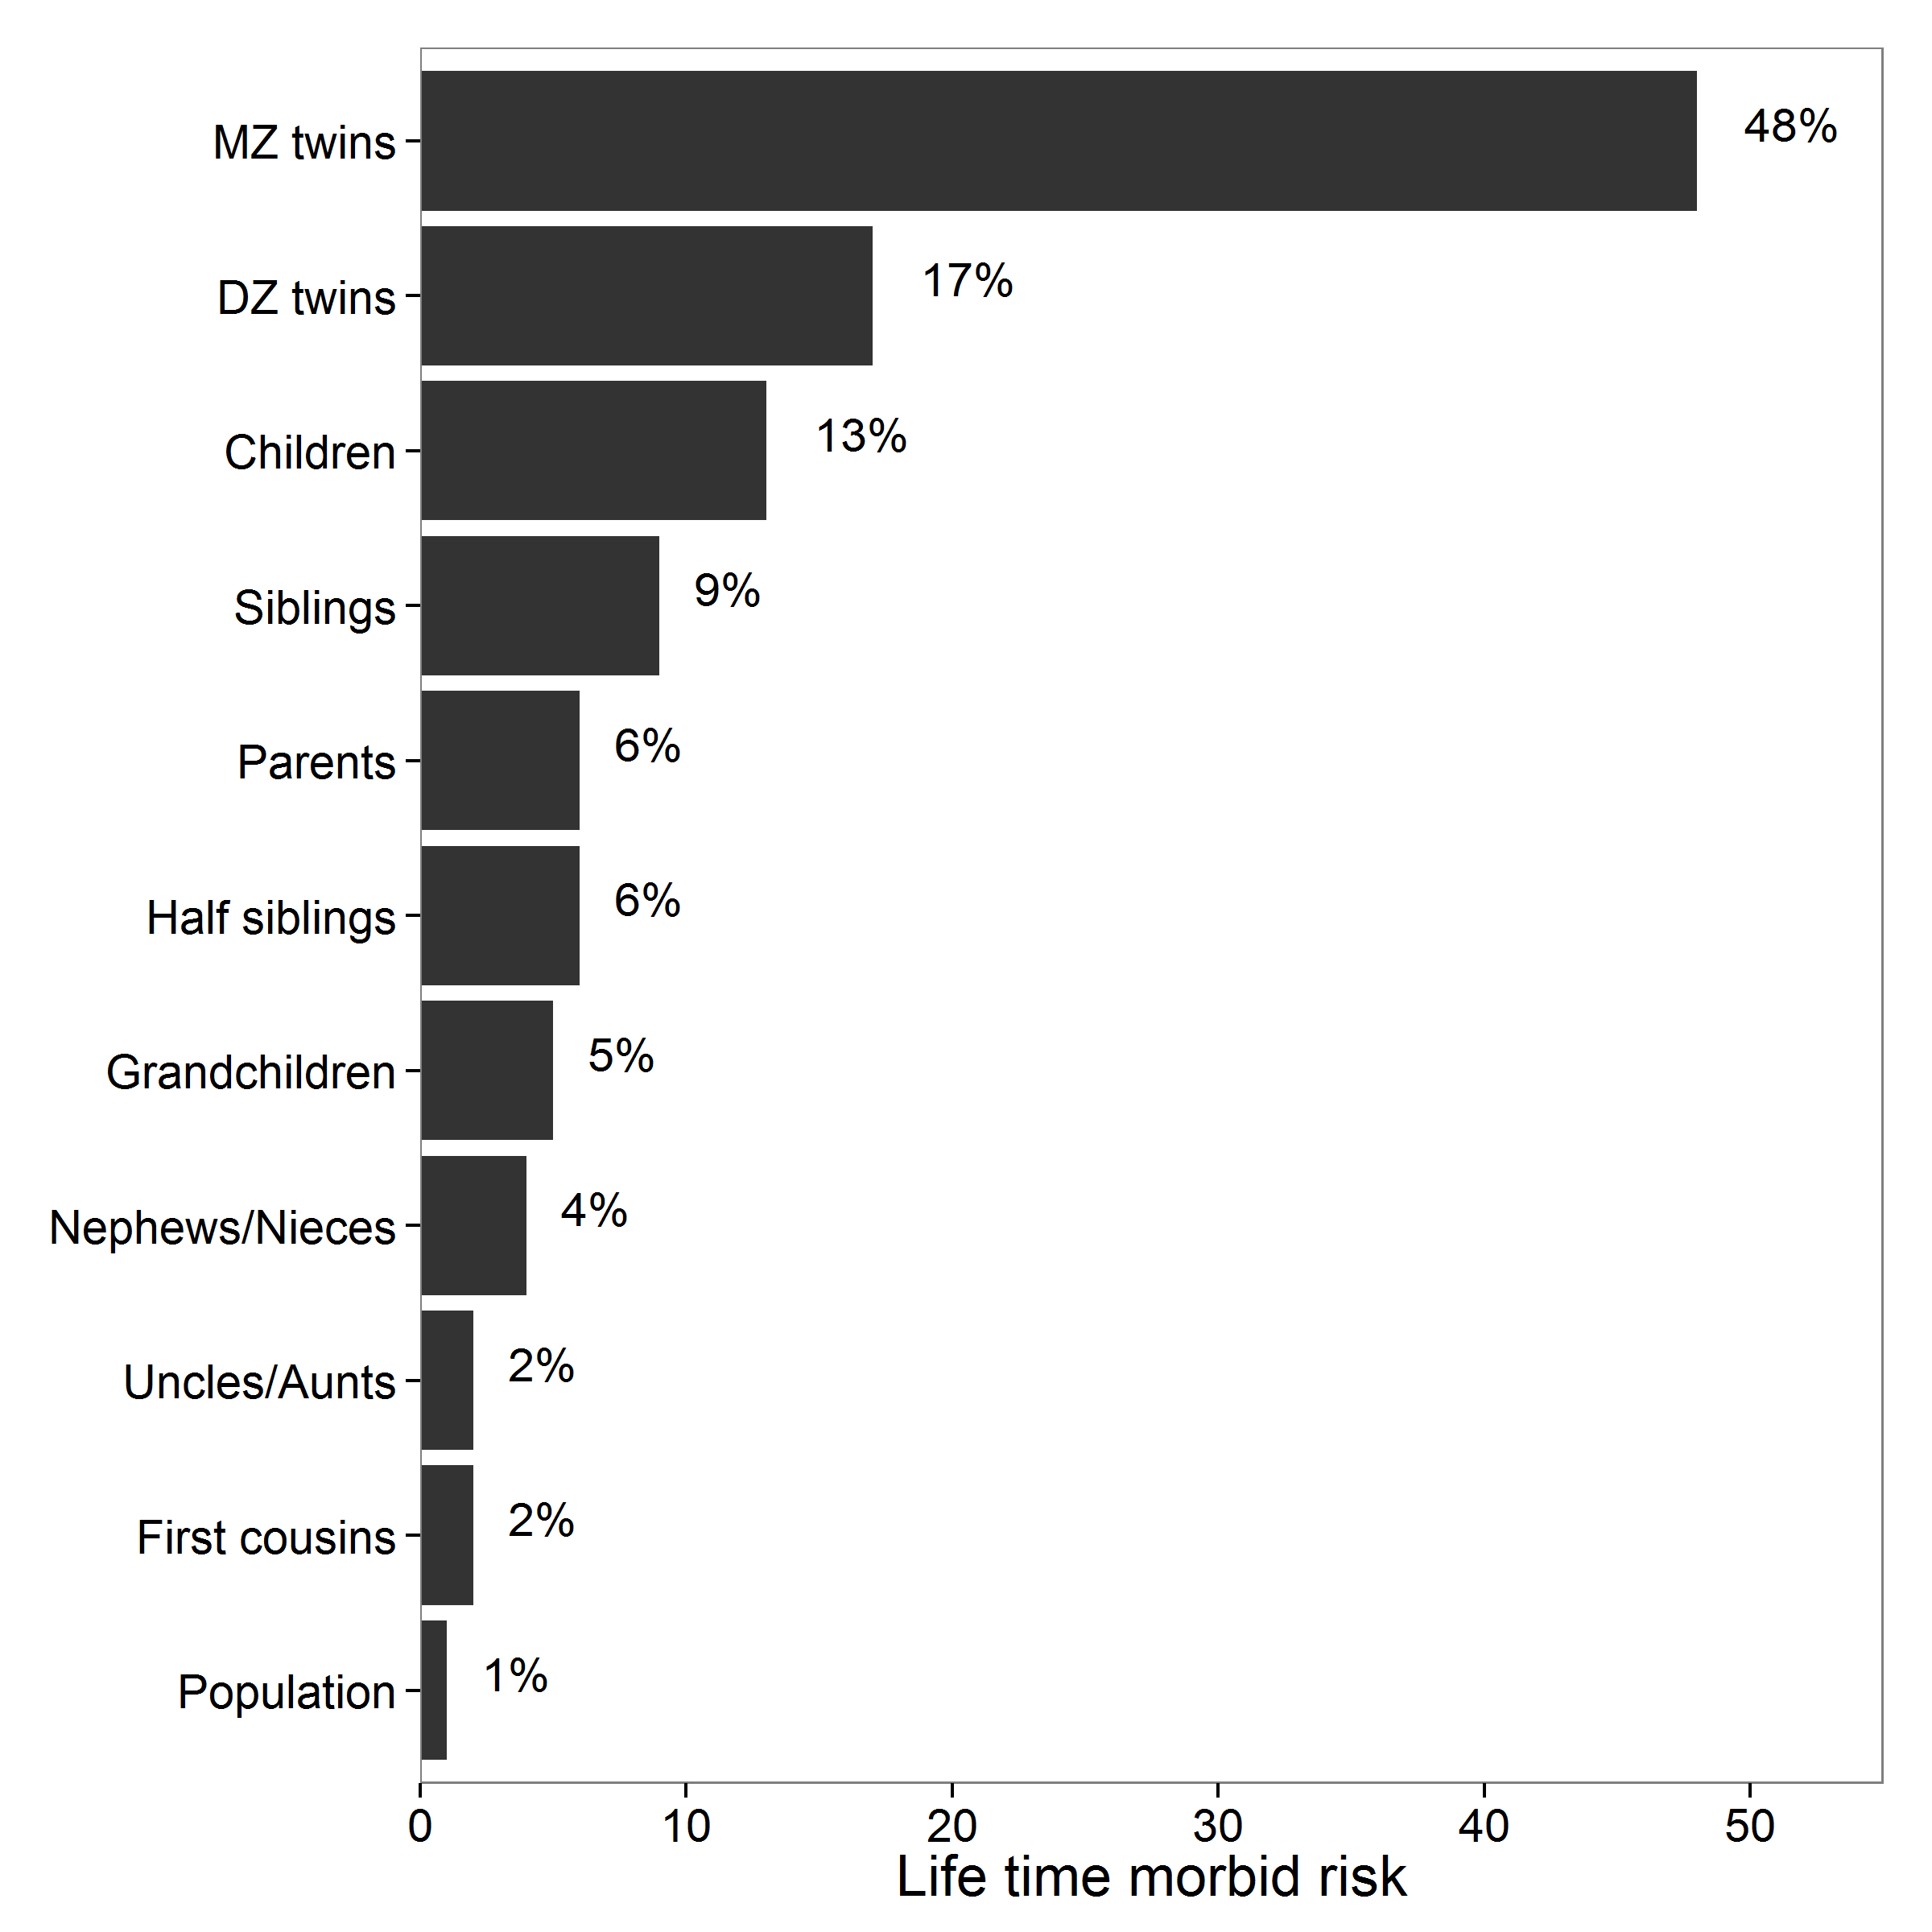
\includegraphics[width=0.5\textwidth]{figure/lifeTimeMorbidRisk.png}
		\caption[Lifetime morbid risks of \glng{scz} in various classes of relatives of a proband]{Lifetime morbid risks of \glng{scz} in various classes of relatives of a proband.
			It was noted that the morbid risk of monozygotic (MZ) twins were only $48\%$, much lower than one would expect if \glng{scz} follows a Mendelian pattern.
			Reproduced with permission from journal\citep{Riley2006}. \label{fig:lifeMRscz}}
	\end{wrapfigure}
	Studies on estimation of heritability of \glng{scz} strongly support \glng{scz} as a genetic disorder.
	However, little was known about the mechanism of \glng{scz} nor the genetic architecture of the disorder. 
	All data from adoption studies, twin studies and family studies shown that \glng{scz} does not follow the Mendelian framework\cite{Gottesman01071967,Gottesman1982}.
	Specifically, shall \glng{scz} be a Mendelian disorder, then we would expect all \gls{mz} siblings of the proband to also suffer from \glng{scz}.
	However, the life time morbid risk of monozyogitc twins were only $48\%$(\cref{fig:lifeMRscz})\citep{gottesman1991schizophrenia}, making it unlikely for \glng{scz} to follow a Mendelian pattern.
	
	Based on these observations, \cite{Gottesman1967} proposed that \glng{scz} follows a polygenic model where disease phenotype were determined by the additive effects from multiple genes.
	Thus, \glng{scz} is a complex genetic disorder with complicated pattern of inheritance. 
	Their hypothesis was supported by the calculation of \cite{Risch1990a} by taking into account of different inheritance model and the life time morbid risk observed in relatives of affected individuals.
	
	Another interesting conclusion from the calculation of \citet{Risch1990a} was the effect size of individual locus. 
	By comparing the observed life time morbid risk and the calculated risk from different models, \citeauthor{Risch1990a} 	suggested that genetic models with a single locus with risk of 3.0 and with all other loci of small effect or models with two or three loci with risk of 2.0 were most consistent with the observed life time morbid risk of \glng{scz}.	\citep{Risch1990}.
	
	\citeauthor{Risch1990a}'s calculation provided an explanation for the early inconsistent findings of linkage studies in \glng{scz}\citep{Harrison2005}.
	As linkage studies were aimed to identify genetic variation of large effect size they failed to capture genetic loci with small effect size.
	It was therefore tempting to suggest that \glng{scz} only follows the ``common disease-common variant'' model, which stated that \glng{scz} should be mediated by large amount of common variants such as \glng{SNP}, each carries a small effect size.
	
	However, another possible hypothesis was that the variation mediating \glng{scz} were rare, therefore require a large sample size to detect. 
	The inconsistent results of the early linkage studies might be due to the inadequate sample size. 
	This lead to some researchers suggesting the ``common disease-rare variant'' hypothesis, which propose that \glng{scz} was mediated by a small amount of rare variants, each with a large effect size\citep{McClellan2007}.
	
	Nevertheless, success in genetic research of \glng{scz} remains limited.
	Only until the initiation of Human Genome Project and the technological advance resulted from the it does genetic research of \glng{scz} entered an era of success.

	\subsection{The Human Genome Project and HapMap Project}
	\glsreset{SNP}
	\glsreset{LD}
	In 1990, the Human genome project was initiated, aiming at constructing the first physical map of the human genome at per nucleotide resolution\citep{Lander2001}.
	The completion of the human genome project has opened up a new era of genetic research, allowing researchers to identify \glspl{SNP} on the human genome, which is one of the major source of genetic variation.
	
	Soon after the completion of the human genome project, the HapMap Project was initiated\citep{Consortium2005}, aiming to provide a genome-wide database of common human sequence variation such as \glspl{SNP} with \gls{maf} $\ge0.05$.
	More importantly was that the HapMap Project also provided a detailed \gls{LD} map of the human genome.
	
	\gls{LD} was of particular importance to genetic research for it was the non-random correlation of genotypes between 2 genetic locus. 
	\glspl{SNP} in high \gls{LD} were usually observed together in the human genome.
	When a large amount of \glspl{SNP} were in high \gls{LD} together, they form what was known as a \gls{LD} block.
	By performing association testing on \glspl{SNP} representing a \gls{LD} block(``tagging''), one can avoid the need of performing association on the whole genome, therefore reducing the cost of the experiment.
	This was the fundamental concept of \gls{GWAS} which tests the 
	which was now extensively used in the genetic research.
	
	\subsection{Genome Wide Association Study}
	In \gls{GWAS}, genome-wide genotyping array were commonly used to systematically detect genetic variants such as \gls{SNP} and \gls{cnv}.
	For quantitative traits, the association between the trait and frequency of the variants were calculated using methods such as linear regression.
	On the other hand, for dichotomous traits such as \glng{scz}, the frequency of the variants were compared between the case and control samples using methods such as chi-square test or logistic regression.
	Because of the problem of multiple testing, only variants with a p-value passing a genome wide threshold (p-value $\le5\times10^{-8}$) were considered significant.
	Another possible method to decide the significant threshold was to consider the ``effective number'' of tests\citep{Li2011} taking into consideration of \gls{LD} as not all tests in a \gls{GWAS} were independent of each other. 
	The power of the \gls{GWAS} were determined by the magnitude of effect, sample size, and required level of statistical significance(the false-positive, or type I, error rate)\citep{Purcell2003}.
	A large sample size and a large effect usually result in a larger power.
	
	\subsubsection{Single Nucleotide Polymorphism} 
	Despite the great promise from \gls{GWAS}, early \gls{GWAS} in \glng{scz} remain largely disappointing and were unable to identify any robust genetic markers associated with \glng{scz}.
	The failure of early \gls{GWAS} in \glng{scz} were mainly due to the relative small sample size of the studies, which result in low detection power.
	
	To overcome the problem of small sample size, large consortium were formed such that data from different research groups from different countries were combined, essentially providing a large sample size for the analysis.
	By 2014, the \Glng{scz} Working group of the \gls{pgc} has collected 34,241 \glng{scz} samples and 45,604 controls\citep{Ripke2014}.
	By combining the samples with those obtained by deCODE genetics, a total of 36,989 \glng{scz} samples and 113,075 controls were used for the largest meta analysis of \glng{scz}.
	In their study\citep{Ripke2014}, 128 linkage-disequilibrium-independent \glspl{SNP} were found to  exceeded the genome-wide significance(p-value $\le 5\times10^{-8}$), corresponding to 108 genetic loci.
	75\% of these loci contain protein coding genes and a further 8\% of these loci were within 20kb of a gene. 
	It was found that genes involved in glutamatergic neurotransmission (e.g. \textit{GRM3}, \textit{GRIN2A} and \textit{GRIA1}), synaptic plasticity and genes encoding the voltage-gated calcium channel subunits (e.g. \textit{CACNA1C}, \textit{CACNB2} and \textit{CACNA1I}) were among the genes associated within these loci.
	Importantly, \textit{DRD2}, the target of all effective anti-psychotic drug were also associated with \glng{scz}.
	This result converges with existing knowledge of \textit{DRD2} being involved in the pathology of \glng{scz}, supported by multiple lines of research\citep{Talkowski2007}.
	\begin{figure}
		\centering
		\caption[Enrichment of enhancers of SNPs associated with Schizophrenia]{Enrichment of enhancers of SNPs associated with \glng{scz}. 
			It was observed that the largest enrichment were in cell lines related to the brain and in tissues with important immune functions. 
			Graphs reproduced with permission from the journal.\citep{Ripke2014}}
		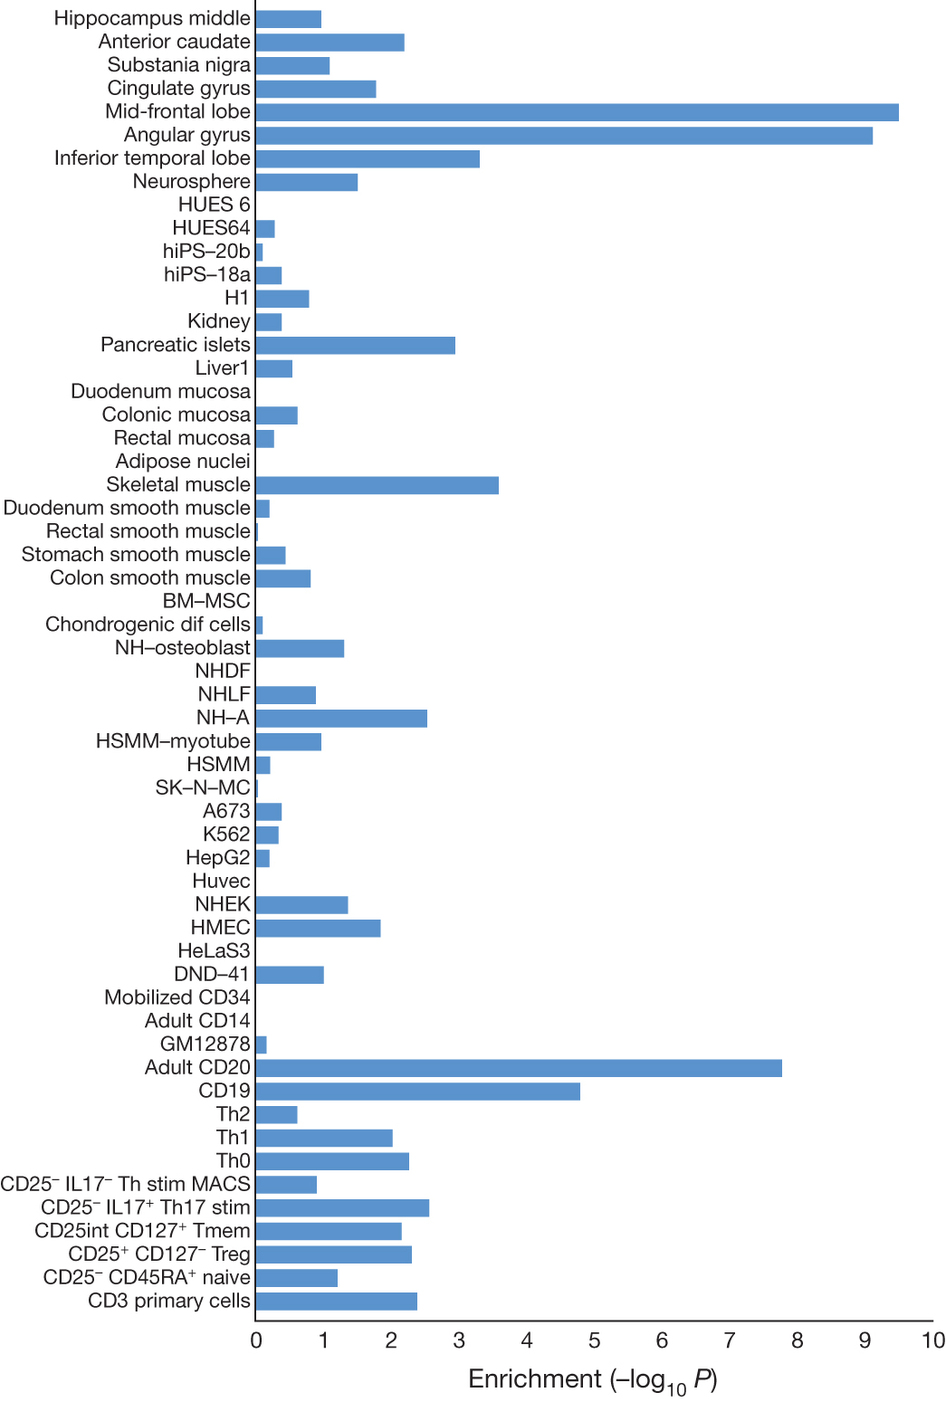
\includegraphics[height=\textwidth]{figure/pgc_enrichment_tissue.jpg}
		\label{fig:pgcEnrich}
	\end{figure}
	It was further demonstrated that \glng{scz} association were significantly enriched at enhancers active in brain and enriched at enhancers active in tissues with important immune functions(\cref{fig:pgcEnrich})\citep{Ripke2014}.
		
	The enrichment of immune related enhancers remains significant even after the removal of \gls{mhc} region from the analysis, provided further genetic support of the involvement of the immune system in the etiology of \glng{scz}.
	Because of its role in neural development\citep{Zhao1998,Deverman2009}, it is likely that the perturbation in the immune system might disrupt the brain development, therefore increasing the risk of \glng{scz}.
	Indeed, studies on \gls{mia} has demonstrated that cytokine imbalance might predispose individual to \glng{scz}\citep{Meyer2009}. 
	
	\subsubsection{Copy Number Variation}
	\glsreset{cnv}
	Another important arm of genetic research in \glng{scz} was to identify \gls{cnv} associated with \glng{scz}.
	\gls{cnv} were classified as segment of DNA that is 1kb or larger and that is present at a different copy number when compared to the reference genome, usually in the form of insertion, deletion or duplication\citep{Feuk2006}.
	Due to the length of these variants, the \gls{cnv} might contain the entire genes and their regulatory regions which might in turn contribute to significant phenotypic differences\citep{Feuk2006}.
	
	To identify robust association between \gls{cnv} and \glng{scz}, \cite{Szatkiewicz2014} conducted a \gls{GWAS} for \gls{cnv} association with \glng{scz} used the Swedish national sample (4,719 \glng{scz} samples and 5,917 controls).
	In their study, they were able to association between \glng{scz} and \gls{cnv} such as 16p11.2 duplications, 22q11.2 deletions, 3q29 deletions and 17q12 duplications were identified.
	Through the gene set association analysis, calcium channel signaling and binding partners of the fragile X mental retardation protein were found to be associated with these \gls{cnv}\citep{Szatkiewicz2014}.
	Interestingly, the calcium channel signaling were also enriched in the \gls{pgc} \gls{GWAS} on \gls{SNP} association, suggesting that the variants were converging on similar set of pathway or gene sets. 
	
	% I need to state rare and large effect because LDSC cannot do that 
	Unlike the result form the \gls{GWAS} on \gls{SNP} data, the \gls{cnv} identified were rare($\le12$ in 4,719 samples) and has a relative large effect (e.g. 22q11 deletion has an odd ratio of 16.32\citep{Szatkiewicz2014}). 
	The results from the \gls{SNP} \gls{GWAS} supports the ``common disease-common variant'' model whereas the \gls{GWAS} on \gls{cnv} supports the ``common disease-rare variant'' model, illustrating the complex genetic model behind the etiology of \glng{scz}.
	
	Although the \gls{GWAS} in \glng{scz} seems to return a lot of interesting results, the question remains: How much of the known genetic risk factors associated explain the disease risk of \glng{scz}?
	To answer these question, we need to estimate the heritability based on the \gls{GWAS} data. 
	However, in order to obtain the large volume of data, most of the samples were not relatives. 
	How can one estimate the heritability based only on the genetic data of the general population instead of family or twin data?
	
	
	\subsection{\glng{gcta}}
	Unlike family based data, the relationship between the samples were unknown. 
	Yet in a typical \gls{GWAS}, the genotype of each individuals were known.
	The ``genetic distance'' between two individual will provide an estimate of their relationship, thus allowing the calculation of heritability.
	\citet{Yang2011} use the concept of genetic distance to calculate the \gls{grm} to represent the relationship between individuals.
	The \gls{grm} were then used in the restricted maximum likelohood analysis(REML) to estimate the heritability of the trait\citep{Yang2011}.
	This was implemented in \gls{gcta} and were now wildly used in the estimation of heritability on \gls{GWAS} data.
	
	The problem with \gls{gcta} was that it require the genotype data to estimate the heritability.
	However, for complex disease like \glng{scz}, the data were usually obtained from multiple data source.
	Because of privacy issues, usually only the test statistic were shared among the research groups and only meta analysis were performed.
	Given there was no raw genotype data, it is impossible to calculate the \gls{grm}, thus making the use of \gls{gcta} impossible.
	  
	\subsection{\glng{ldsc}}
	Sometimes, in a \gls{GWAS} study, one can observe an general inflation of test statistics. 
	It was usually considered to be contributed to the presence of confounding factors such as population stratification under the assumption that most of the \glspl{SNP} should have no association to the disease.
	It was therefore a common practice for one to perform the \gls{gc} on the \gls{GWAS} results\citep{Zheng2006}.
	
	The problem of the \gls{gc} was that the basic assumption of a small number of causal \glspl{SNP} might not be true. 
	Through careful simulation, \citet{Yang2011b} demonstrated that in the absence of population stratification and other form of technical artifacts, the presence of polygenic inheritance can also inflate the test statistic\citep{Yang2011b}.
	More importantly, they observed that the magnitude of inflation was determined by the \emph{heritability}, the \gls{LD} structure, sample size and the number of causal \glspl{SNP} of the trait.

	Following on this observation, \citet{Bulik-Sullivan2015} developed the \gls{ldsc}.
	The fundamental concept of \gls{ldsc} was that the more genetic variant a \gls{SNP} tag, the more likely for it to be able to tag a causal variant; 
	whereas population stratification and cryptic relatedness should not be associated with \gls{LD}.
	The number of genetic variants tagged by a \gls{SNP}$_j$ ($l_j$)(\gls{LD} score) was then defined as the sum of $r^2$ of the $k$ \glspl{SNP} within a 1cM window of \gls{SNP}$_j$:
	\begin{equation}
	l_j = \sum_kr^2_{jk}
	\label{eq:ldScore}
	\end{equation}
	
	The expected $\chi^2$ of \gls{SNP}$_j$ was then defined as a function of the \gls{LD} score ($l_j$), the number of samples ($N$), the number of \glspl{SNP} in the analysis($M$), the contribution of confounding factors ($a$) and most importantly, the heritability ($h^2$):
	\begin{equation}
	\mathrm{E}[\chi^2_j | l_j] = \frac{Nl_jh^2}{M}+Na+1
	\label{eq:fullLDSC}
	\end{equation}
	If one express the \gls{LD} score and the $chi^2$ as vectors $\boldsymbol{L}$ and $\boldsymbol{\chi^2}$ respectively, \cref{eq:fullLDSC} becomes a regression of the $\chi^2$ against the \gls{LD} score:
	\begin{equation}
	\boldsymbol{\chi^2}= \frac{N}{M}\boldsymbol{L}h^2+Na+1
	\label{eq:ldReg}
	\end{equation}
	
	As a result of that, the heritability $h^2$ will be the slope of the regression and the intercept minus one will represent the mean contribution of the confounding bias such as those of population stratification. 
	Thus, \cref{eq:ldReg} can be used for the estimation of heritability given only the test statistics and the population \gls{LD} were provided. 
	
	
	Using data from \citet{Ripke2014}, and applying the liability threshold adjustment, \citet{Bulik-Sullivan2015} estimated the heritability of \glng{scz} should be 0.555 with \gls{se} of 0.008.
	The estimated heritability was lower than what was previously estimated from population based study(64\%\citep{Lichtenstein2009}) and twin studies(81\%\citep{Sullivan2003}).
	Possible reasons of such discrepancies might be that in \citet{Ripke2014}'s study, only \glspl{SNP} data were collected. 
	From \citet{Szatkiewicz2014}, it was clearly demonstrated that other than \glspl{SNP}, \glspl{cnv} were also associated with \glng{scz}.
	By ignoring \glspl{cnv} in the estimation of heritability, the estimation of \citet{Bulik-Sullivan2015} would only provided a lower bound of heritability estimated.
	Another possibility of the``missing'' heritability can be due to interaction between the genetic and environmental factors. 
	Although previous studies\citep{Gottesman01071967} suggested that the non-additive genetic factors were unlikely to contribute to \glng{scz}, the possibility of involvement of gene-environmental interaction $G\times E$ were not ruled out.
	Indeed, in the adoption study conducted by \citet{Tienari2004}, it was found that individuals with higher genetic risk were significantly more sensitive to ``adverse'' vs ``healthy'' rearing patterns in adoptive families than are adoptees at low genetic risk\citep{Tienari2004}, providing support to a possible interaction between genetic and environmental factors.
	Therefore, in order to account for the ``missing'' heritability, one might need to consider genetic variations other than \glspl{SNP} and might need to take into consideration of the $G\times E$ interaction.
	
	Nonetheless, the heritability estimation from \citet{Ripke2014} were still encouraging, as for the first time in genetic research of \glng{scz}, a large portion of heritability of \glng{scz} were finally identified.
	This permit the genetic research of \glng{scz} to move beyond statistical association and focus on the functional basis of the genetic susceptibility locus of \glng{scz}.
	
	\subsection{Partitioning of Heritability of Schizophrenia}
	\subsectionmark{Partitioning of Heritability}
	Traditionally, functional enrichment analysis in \gls{GWAS} only take into account of \glspl{SNP} that passed the genome wide significance threshold. 
	However, for complex traits such as that of \glng{scz}, much fo the heritability might lies in \glspl{SNP} that do not reach genome wide significance threshold at the current sample size.
	For example, in 2013, only 13 risk loci were detected using 13,833 \glng{scz} samples and 18,310 controls \citep{Ripke2013}. 
	When the sample size increased to 34,241 \glng{scz} samples and 45,604 controls in 2014, 108 risk loci were identified\citep{Ripke2014}. 
	Thus, if one only consider the significant loci, risk loci that have not reach genome wide significance threshold might be ignored from the analysis, decreasing the power of the functional enrichment analysis.
	
	Unlike traditional functional enrichment analysis, \gls{ldsc} uses information from all \glspl{SNP} and taking into account of the \gls{LD} structure to partition heritability into different functional categories. 
	Thus should be more powerful when compared to traditional analysis and should help to provide useful insight into the disease etiology of \glng{scz}.

	\citet{Finucane2015} used data from \citet{Ripke2014} and functional categories derived from the ENCODE annotation\citep{ENCODEProjectConsortium2012}, the NIH Roadmap Epigenomics Mapping Consortium annotation\citep{Bernstein2010} and other studies\citep{Finucane2015}, it was found that the brain cell types were most enriched in \glng{scz}, especially those related to the \gls{cns}.
	Of all the functional categories, the most enriched category in \glng{scz} was the H3K4me3 mark in the fetal brain(\cref{tab:cellTypeScz}). 
	As H3K4me3 was mostly linked to active promoters, it was likely for genes that were active in fetal brain (e.g genes related to brain development) to be associated with \glng{scz}, supporting the idea of \glng{scz} as an neuro-developmental disorder. 
	
	Moreover, it was also observed that the second most enriched cell types were those related to immunity.
	Undoubtedly, the \gls{cns} and the immune system have an important role in the disease etiology of \glng{scz}. 

	\begin{singlespace}
	\begin{longtable}{p{6cm}rrr}
		%\begin{tabular}{rrrr}
			\toprule
			Cell type & cell-type group & Mark  & P-value \\
			\midrule
			Fetal brain** & CNS   & H3K4me3 & $3.09\times 10^{-19}$ \\
			Mid frontal lobe** & CNS   & H3K4me3 & $3.63\times 10^{-15}$ \\
			Germinal matrix** & CNS   & H3K4me3 & $2.09\times 10^{-13}$ \\
			Mid frontal lobe** & CNS   & H3K9ac & $5.37\times 10^{-12}$ \\
			Angular gyrus** & CNS   & H3K4me3 & $1.29\times 10^{-11}$ \\
			Inferior temporal lobe** & CNS   & H3K4me3 & $1.70\times 10^{-11}$ \\
			Cingulate gyrus** & CNS   & H3K9ac & $5.37\times 10^{-11}$ \\
			Fetal brain** & CNS   & H3K9ac & $5.75\times 10^{-11}$ \\
			Anterior caudate** & CNS   & H3K4me3 & $2.19\times 10^{-10}$ \\
			Cingulate gyrus** & CNS   & H3K4me3 & $4.57\times 10^{-10}$ \\
			Pancreatic islets** & Adrenal/Pancreas & H3K4me3 & $2.24\times 10^{-09}$ \\
			Anterior caudate** & CNS   & H3K9ac & $3.16\times 10^{-9}$ \\
			Angular gyrus** & CNS   & H3K9ac & $4.68\times 10^{-9}$ \\
			Mid frontal lobe** & CNS   & H3K27ac & $7.94\times 10^{-9}$ \\
			Anterior caudate** & CNS   & H3K4me1 & $1.20\times 10^{-8}$ \\
			Inferior temporal lobe** & CNS   & H3K4me1 & $3.72\times 10^{-8}$ \\
			Psoas muscle** & Skeletal Muscle & H3K4me3 & $4.17\times 10^{-8}$ \\
			Fetal brain** & CNS   & H3K4me1 & $6.17\times 10^{-8}$ \\
			Inferior temporal lobe** & CNS   & H3K9ac & $9.33\times 10^{-8}$ \\
			Hippocampus middle** & CNS   & H3K9ac & $9.33\times 10^{-7}$ \\
			Pancreatic islets** & Adrenal/Pancreas & H3K9ac & $1.62\times 10^{-6}$ \\
			Penis foreskin melanocyte primary** & Other & H3K4me3 & $2.09\times 10^{-6}$ \\
			Angular gyrus** & CNS   & H3K27ac & $2.34\times 10^{-6}$ \\
			Cingulate gyrus** & CNS   & H3K4me1 & $2.82\times 10^{-6}$ \\
			Hippocampus middle** & CNS   & H3K4me3 & $2.82\times 10^{-6}$ \\
			CD34 primary** & Immune & H3K4me3 & $4.68\times 10^{-6}$ \\
			Sigmoid colon** & GI    & H3K4me3 & $5.01\times 10^{-6}$ \\
			Fetal adrenal** & Adrenal/Pancreas & H3K4me3 & $6.31\times 10^{-6}$ \\
			Inferior temporal lobe** & CNS   & H3K27ac & $8.32\times 10^{-6}$ \\
			Peripheralblood mononuclear primary** & Immune & H3K4me3 & $9.33\times 10^{-6}$ \\
			Gastric** & GI    & H3K4me3 & $1.17\times 10^{-5}$ \\
			Substantia nigra* & CNS   & H3K4me3 & $1.95\times 10^{-5}$ \\
			Fetal brain* & CNS   & H3K4me3 & $2.63\times 10^{-5}$ \\
			Hippocampus middle* & CNS   & H3K4me1 & $3.31\times 10^{-5}$ \\
			Ovary* & Other & H3K4me3 & $6.46\times 10^{-5}$ \\
			CD19 primary (UW)* & Immune & H3K4me3 & $7.08\times 10^{-5}$ \\
			Small intestine* & GI    & H3K4me3 & $8.51\times 10^{-5}$ \\
			Lung* & Cardiovascular & H3K4me3 & $1.17\times 10^{-4}$ \\
			Fetal stomach* & GI    & H3K4me3 & $1.29\times 10^{-4}$ \\
			Fetal leg muscle* & Skeletal Muscle & H3K4me3 & $1.51\times 10^{-4}$ \\
			Spleen* & Immune & H3K4me3 & $1.70\times 10^{-4}$ \\
			Breast fibroblast primary* & Connective/Bone & H3K4me3 & $2.04\times 10^{-4}$ \\
			Right ventricle* & Cardiovascular & H3K4me3 & $2.14\times 10^{-4}$ \\
			CD4+ CD25- Th primary* & Immune & H3K4me3 & $2.19\times 10^{-4}$ \\
			CD4+ CD25- IL17- PMA Ionomycin stim MACS Th sprimary* & Immune & H3K4me1 & $2.19\times 10^{-4}$ \\
			CD8 naive primary (UCSF-UBC)* & Immune & H3K4me3 & $2.24\times 10^{-4}$ \\
			Pancreas* & Adrenal/Pancreas & H3K4me3 & $2.34\times 10^{-4}$ \\
			CD4+ CD25- Th primary* & Immune & H3K4me1 & $2.75\times 10^{-4}$ \\
			CD4+ CD25- CD45RA+ naive primary* & Immune & H3K4me1 & $2.75\times 10^{-4}$\\
			Colonic mucosa* & GI    & H3K4me3 & $3.24\times 10^{-4}$ \\
			Right atrium* & Cardiovascular & H3K4me3 & $3.31\times 10^{-4}$ \\
			Fetal trunk muscle* & Skeletal Muscle & H3K4me3 & $3.39\times 10^{-4}$ \\
			CD4+ CD25int CD127+ Tmem primary* & Immune & H3K4me3 & $3.47\times 10^{-4}$ \\
			Substantia nigra* & CNS   & H3K9ac & $3.63\times 10^{-4}$ \\
			Placenta amnion* & Other & H3K4me3 & $4.17\times 10^{-4}$ \\
			Breast myoepithelial* & Other & H3K9ac & $5.50\times 10^{-4}$ \\
			CD8 naive primary (BI)* & Immune & H3K4me1 & $5.75\times 10^{-4}$ \\
			Substantia nigra* & CNS   & H3K4me1 & $6.61\times 10^{-4}$ \\
			Cingulate gyrus* & CNS   & H3K27ac & $7.94\times 10^{-4}$ \\
			CD4+ CD25- CD45RA+ naive primary* & Immune & H3K4me3 & $8.71\times 10^{-4}$ \\
			\bottomrule
		%\end{tabular}%
		\caption[Enrichment of Top Cell Type of Schizophrenia]{Enrichment of Top Cell type of Schizophrenia.
			* = significant at False Discovery Rate $<$ 0.05.
			** = significant at p $<$ 0.05 after correcting for multiple hypothesis. 
			Reproduce with permission from Journal.\citep{Finucane2015}}
		\label{tab:cellTypeScz}%
	\end{longtable}%
	\end{singlespace}
	
	\subsection{Genetic Correlation}
	Another very important application of \gls{ldsc} is that it allow one to identify the genetic correlation between traits\citep{Bulik-Sullivan2015a}. 
	The genetic correlation can be used as an genetic analogue to co-morbidity, thus allowing deeper understanding to the etiology of the traits.
	Above all, genetic correlation was important in studying the treatment response. 
	It has been observed that there was an increased prevalence of anxiety, depression and substance abuse in \glng{scz}\citep{Buckley2009}. 
	These co-morbidity were generally associated with more severe psychopathology and with poorer outcome\citep{Buckley2009}.
	A deeper understanding of possible co-morbidity between different traits and \glng{scz} might provide insight not only to the disease etiology of \glng{scz}, it might even provide important information in possible treatment options for \glng{scz}. 
	Using breast cancer as an example, it was found that patients with comorbidity had poorer survival than those without comobidity\citep{Sogaard2013} and it was suggested that by treating the comorbid diseases, one might be able to delay mortality in breast cancer patients\citep{Ording2013}.
		
	By applying their method to 25 different phenotypes, \citet{Bulik-Sullivan2015a} shown that \glng{scz} has significant genetic correlation with bipolar disorder, major depression and more surprisingly, anorexia nervosa.
	Previous studies have always suggest there to be an co-morbidity between \glng{scz} and bipolar disorder \citep{Lichtenstein2009,Purcell2009,Buckley2009}.
	Similarly, it was not uncommon for \glng{scz} to display depressive symptoms\citep{Buckley2009}. 
	It was even observed that individuals at high risk and ultrahigh risk for developing \glng{scz} have generally demonstrated a significant degree of depressive symptoms prior to and during the emergence of psychotic symptoms, suggesting a close relationship between \glng{scz} and depression. 
	
	On the other hand, the genetic correlation between \glng{scz} and anorexia nervosa were slightly unexpected for there has been a lack of study in the co-morbidity between eating disorder and \glng{scz}. 
	Nonetheless, this finding raises the possibility of similarity between anorexia and nervosa.
	% Serotonergic system have been implicated in depression, negative symptoms of sczhiophrneia and eating disorders \citep{Arranz2007}.
	%	\section{Antipsychotics}
	Despite the success in the genetic research of \glng{scz}, an effective cure of \glng{scz} was yet to be found.
	Currently, the main treatment method for \glng{scz} was the use of antipsychotic drugs to reduce symptoms and prevent relapse. 
	However, there was a large variability between individuals in their response to treatment, some might even suffer from adverse side effects such as agranulocytosis and \gls{td}.
	Thus, it is vital to administrate the antipsychotics according to individual conditions.
	Unfortunately, there was an lack of understanding of the factors influencing the drug response, forcing clinicians to administrate antipsychotics on a trial and error process.
	There is a therefore a pressing need for better understanding treatment response in \glng{scz} such that an optimal treatment can be provided for the patients.
	
	\subsection{History of Antipsychotic}
	Early research in treatment of \glng{scz} largely follows a random trial and error process where methods such as prolonged sleep treatment, insulin coma therapy and pharmacoconvulsive treatment were proposed\citep{Lehmann1997}.
	The first antipsychotic drug Chlorpromazine, a phenothiazine, were developed in early 1950s.
	Subsequently within a period of less than 10 years, 20 other antipsychotic phenothiazine were in development.
	Collectively, they were considered as the \glspl{fga}.
	
	\glspl{fga} were found to be extremely effective in reducing the positive symptoms of schizophrenia such as delusions, hallucinations and disorganized thinking.
	However, the \glspl{fga} were found to be ineffective against negative and cognitive symptoms, and might even cause acute \gls{eps} such as parkinsonism, dysphoria and tardive dyskinesia, making them unpopular among patients\citep{Tandon2007}.
	
	In 1966, a new drug, name Clozapine was introduced\citep{Lehmann1997}. 
	Clozapine has been shown to be more effective when compared to \glspl{fga} and was less likely to cause \gls{eps} and tardive dyskinesia.
	Moreover, it was shown to reduce suicidality and was more effective in reducing negative and cognitive symptoms\citep{Lehmann1997,Tandon2007}.
	Despite the superior performance of Clozapine, it found to be associated with the severe and potentially lethal adverse side effect, agranulocytosis\citep{Alvir1993}, limiting its use as a first line treatment of \glng{scz}\citep{Remington2013}.
	Subsequently, a number of antipsychotic were developed in hope of a ``safe clozapine'' which have the same level of effectiveness as clozapine and not having the adverse side effects.
	These were considered as the \glspl{sga} which includes risperidone, olanzapine and quetiapin.
	Although the \glspl{sga} tends to have lower risk for \gls{eps}, they tends to be associated with significant metabolic side effects such as weight gain, diabetes mellitus and hyperlipidemia\citep{UCOK2008}.
	
	\subsection{Mechanism of Action of Antipsychotic}
	The difference between the \glspl{fga} and \glspl{sga} provides valuable information on possible mechanisms associated with treatment response and adverse side effects such as \gls{eps}.
	It was first demonstrated on 1963 that \glspl{fga} tends to block the dopamine receptors\citep{Lehmann1997} and it was hypothesized that the binding of dopamine receptors, especially the D$_2$ receptors were required for reduction of positive symptoms\citep{Arranz2007}. 
	Indeed, it was found that dopamine receptor blockade was not unique to \glspl{fga} but was also required for \glspl{sga} and there has yet been any successful antipsychotic drugs that works without dopamine D$_2$ blockade\citep{Zhang2011}.
	However, it was observed that there were significant differences between \glspl{fga} and \glspl{sga} affinities. 

	When compared to \glspl{fga}, \glspl{sga} have a lower affinity for and occupancy at the D$_2$ receptors and tends to have a more diverse receptor binding profiles.
	For example, the ratio between affinity of serotonin receptor (5-HT$_2$) to that of the D$_2$ receptor were significantly greater (15.8 times) for \glspl{sga} when compared to \glspl{fga}\citep{Meltzer1991}.
	These leads to two competing hypothesis of antipsychotic action: 
	the serotonin-dopamine hypothesis, which stated that the ratio of serotonin 5-HT$_2$ to dopamine D$_2$ affinity was the main mechanism accounting for the superior performance of \glspl{sga};
	and the dopamine hypothesis which stated that the modulation of the dopamine D$_2$ receptor was the single most important factor affecting the performance of the antipsychotic\citep{Kapur2003}.
	
	One common characteristics for most \glspl{sga} except amisulpride was their affinity to the serotonin receptors such as 5-HT$_2$. 
	It was therefore suggested that the reduction of negative symptoms were resulting from the serotonin blockade and the serotonin-dopamine interactions were important to the antipsychotic drug actions\citep{Meltzer1999}.
	However, amisulpride serves as a counter example to the serotonin-dopamine hypothesis.
	Amisulpride is a \gls{sga} that does not have any affinity for serotonin receptors yet have comparable performance in reduction of negative response when compared to olanzapine\citep{Kumar2014}.
	Thus, serotonin receptor blockade might not be required for the reduction of negative symptoms.
	
	% Serotonin -> SGA all bind better at serotonin when compared to Dopamine
	Moreover, \gls{pet} studies have shown that a minimum occupancy of 60\%-65\% of striatal D$_2$ like receptors is required to obtain clinical response whereas D$_2$ occupancy of above 80\% is considered as the main cause of \gls{eps}\citep{Arranz2007,Kapur2003}.
	Upon further investigation, it was found that clozapine preferentially target the mesolimbic dopamine system while sparing the nigrostriatal dopamine system\citep{Gardner1993}.
	This raise the possibility that the main difference between \glspl{fga} and \glspl{sga} was the preferential blockade of cortical dopamine D$_2$ receptors compared with striatal dopamine D$_2$ recptors\citep{Kapur2003}.
	Based on these observation, it was now hypothesized that \glng{scz} was a result of both ``hypodopaminergia'' in the prefrontal cortex and ``hyperdopaminergia'' in the straitum, with a possible involvement of the glutamate system\citep{Howes2009}.
	
	It was worth noting that most clinical studies of \glspl{sga} were sponsored by industry, leading to questions of their validity. 
	Two government lead clinical trial, \gls{catie}\citep{Lieberman2005} and CUtLASS\citep{Jones2006}, were therefore performed to provide unbiased comparison between \glspl{fga} and \glspl{sga}.
	Unfortunately, the superior performance of \glspl{sga} over \glspl{fga} were not observed nor were the \glspl{sga} associated with better cognitive or social outcomes.
	It therefore seems like the only advantages of \glspl{sga} over \glspl{fga} were the reduced risk of adverse side effects such as \gls{eps} and \gls{td}.
	
	\subsection{Antipsychotic Response}
	Although the government lead studies does not support \glspl{sga}'s role in reducing negative and cognitive symptoms of \glng{scz}, there is without doubt that \glspl{sga} were better in terms of reduced risk of \gls{eps} and \gls{td}. 
	There is no question that a better treatment is required yet it is just as important to learn how to better utilize currently available antipsychotics. 
	Simply a better understanding of factors behind the variation in individual responses to different antipsychotic drugs will be extremely beneficial. 
	It will allow researchers to categorize people by their personal profile and provide the most optimal antipsychotic drug for their treatment. 
	
	\subsubsection{Positive and Negative Symptom Scale (PANSS)}		
	In order to study the response of antipsychotic, it is important to have an objective scale to quantify the reduction of symptoms.
	The \gls{panss}\citep{Kay1987} were among one of the most commonly scale used to measure the core symptoms of \glng{scz} and is composed of 3 subscales: positive, negative and general psychopathology.
	There were a total of 30 different symptoms included in \gls{panss} and each symptoms were rated from 1 to 7, thus the minimal score for \gls{panss} is 30.
	To calculate the percentage reduction of \gls{panss}, which represent a reduction in severity of symptoms, the reduction of \gls{panss} will then be divided by the original \gls{panss} minus 30:
	$$
		\%\text{improvement} = \frac{\text{PANSS}_{after}-\text{PANSS}_{before}}{\text{PANSS}_{before}-30}\times 100\%
	$$
	
	\subsubsection{Factors Associated with Antipsychotic Responses}
	Factors such as diet, smoking and concomitant medications were known to significantly affect metabolic enzyme activity rates, thus have an impact to antipsychotic treatment response\citep{Arranz2011}.
	On the other hand, clinical features such as treatment adherence and duration of illness; individual variation such as gender and ethnicity all influence the treatment efficacy\citep{Arranz2011}.
	 
	Considering the heritability of \glng{scz} were up to 80\%, genetic variations can explain much of the variation in \glng{scz}. 
	Therefore, people hypothesize that the genetic variations might also be able to explain much of the variation in antipsychotic drug response.
	However, although there were incidence report of concordance of response in \gls{mz} twin data\citep{Vojvoda1996,Mata2001}, the sample size were not enough for heritability estimation(studies usually consist of only one pair of twins).
	Nonetheless, these studies shades lights on the possibility that variation in antipsychotic response might be able to be explained by genetic variations of individuals.
	

	\subsection{Pharmacogenetics and Pharmacogenomics}
	Given that genetic variations might be able to explain the variation in antipsychotic drug response, it was therefore compelling to study the association between genetic variations and antipsychotic drug response.
	The terms ``pharmacogenetics'' and ``pharmacogenomics'' were introduced to define study of variability in drug response due to genetic variations and can be used interchangeably\citep{Pirmohamed2001}. 
	Before the popularity of \gls{GWAS}, pharmacogenetic studies were mainly conducted based on the candidate gene approach.
	Genes targeted by antipsychotic drugs such as genes coding for dopamine receptors and serotonin receptors were among the major target of research.
	Similarly, genes involve in the metabolizing the antipsychotic drugs such as the P450 family of enzymes were extensively studied.
	\subsubsection{Dopamine Receptors}
	The dopamine D$_2$ receptor plays a critical role in antipsychotic drug action, with D$_2$ receptor antagonism considered to be necessary and sufficient for antipsychotic drug efficacy\citep{Kapur2003}.
	As such, polymorphisms on the \textit{DRD2} gene, which codes for the D$_2$ receptor, were extensively studied. 
	The \gls{SNP}(rs1799732) representing a deletion at position -141, which was located in the 5' promoter region of \textit{DRD2} were found to be able to influence the density of D$_2$ receptor density in the striatum in healthy samples unexposed to antipsychotic drug treatment\citep{Arinami1997}.
	A significant difference in response rate between deletion carrier and patients with homozygous insertion genotype were observed (odds ratio = 0.65, 95\% \gls{ci}: 0.43-0.97), indicating patients who carry one or two deletion allele were more likely to have less favorable antipsychotic drug responses.

	Other than the D$_2$ receptor, most antipsychotics also shown similar affinity for the dopamine D$_3$ receptor\citep{Sokoloff2006}, leading to pharmacogenetic studies of variants on the \textit{DRD3} gene, which codes for the D$_3$ receptors.
	Much of the research were focused on the \gls{SNP}(rs6280) coding for the serine to glycine substitution at amino acid position 9 in the N-terminal extracellular domain of the D$_3$ receptor protein.
	It was suggested that the dopamine has 4-5 times higher affinity to the glycine-9 variant when compared to the serine-9 variant\citep{Jeanneteau2006}, thus it was hypothesized that the serine to glycine substitution might modulate the antipsychotic drug response. 
	Interestingly, it was found that the serine allele was associated with better response to \glspl{fga} but was associated with non-repsonse to clozapine treatment\citep{Zhang2011}. 
	However, this finding was not replicated and there was yet any consistent evidence of the association of the serine to glycine substitution with antipsychotic response\citep{Zhang2011}.
	
	\subsubsection{Serontonin Receptors}
	Serontonin receptors, especially the 5-HT$_{2A}$ receptors first gain attention because of it critical involvement in the pathophysiology of hallucinations\citep{Aghajanian1999}, leading to speculation of its role in the etiology of \glng{scz} where hallucinations is one of the main symptoms.
	Although there are debates on the importance of serontonin receptors in antipsychotic drug responses\citep{Kapur2003}, pharmacogenetic studies on serotonin receptors such as the 5-HT$_{2A}$ receptors remains popular.
	
	Polymorphisms on \textit{HTR2A} gene, which codes for the 5-HT$_{2A}$ receptors, were extensively studied. 
	The synonymous \gls{SNP} at codon 10(T102C,rs6313) and the A-1438G \gls{SNP}(rs6311) in the promoter region of \textit{HTR2A} are in complete \gls{LD}. 
	It was found that the C allele of the T102C \gls{SNP}, together with the G allele of the A-1438G \gls{SNP} might cause lower promoter activities of \textit{HTR2A} and may decrease the 5-HT$_{2A}$ densities in some brain areas\citep{Zhang2011}.
	However, results from studies on the association of T102C and A-1438G have not reach an agreement\citep{Zhang2011}.
	
	\subsubsection{Cytochrome P450 enzymes}
	There are many other factors that might affect the antipsychotic drug response.
	For example, the time course of the absorption, the bioavailability, the distribution of the drug in the body, the excretion of the drugs and the metabolism of the drugs all influences the efficacy of antipsychotics.
	Genetic variants in enzymes mediating these factors are therefore interesting target for pharmacogenetic studies.
	
	The Cytochrome P450 enzyme family, including CYP1A1, CYP2A6, CYP2C8,
	CYP2C9, CYP2C19, CYP2D6, CYP2E1, CYP3A5 and many others,  in the liver is one of the major target of pharmacogenetic studies because of its role in metabolizing many of the antipsychotic drugs\citep{Cacabelos2011}.
	Around 40\% of antipsychotics are major substrate for CYP2D6\citep{Cacabelos2011} making it an ideal target to study.
	There are more than 100 genetic variations observed on the \textit{CYP2D6} gene and by combining different alleles, the CYP2D enzyme can be categorized based on the degrees of the enzymatic activities: poor metabolizer, intermediate metabolizer, extensive metabolizer(normal) and ultra-rapid metabolizer\citep{Zhang2011}.
	It was hypothesized that individuals' CYP2D enzymatic activities can affect the level of drugs in their blood. 
	For example, people with \textit{CYP2D} alleles from the poor metabolizer categories were expected to have a higher drug levels in the blood when compared to people with \textit{CYP2D} alleles from the ultra-rapid metabolizer categories.
	
	Although there were data suggesting the association of poor metabolizer with higher rate of drug induced side effects\citep{Ravyn2013}, most studies to date have been unable to provide sufficient evidence to support the use of Cytochrome 450 genotype testing to improve therapeutic
	efficacy in the use of antipsychotic medications\citep{Ravyn2013}.
	However, \citet{Ravyn2013} do agree that the use of cytochrome 450 genotype testing might help to prevent adverse side effects in patients receiving some antipsychotics such as Risperidone and Aripiprazole.
	
	\subsubsection{Genome Wide Association of Antipsychotic Drug response}
	Despite the usefulness of the candidate gene approach, it was restricted by our limited knowledge regarding the mechanism behind antipsychotic response.
	With the popularization of \gls{GWAS} and advancement of sequencing technology, we now have the ability to perform association on variants across the whole human genome, allowing a hypothesis free approach.
	
	The \gls{catie} project conducted a total of four \gls{GWAS}, on phenotype such as antipsychotic treatment response\citep{McClay2011}, antipsychotic-induced
	parkinsonism\citep{Alkelai2009}, movement related adverse antipsychotic effect\citep{Aberg2010} and metabolic side effects\citep{Adkins2011}.
	For the study of antipsychotic treatment response\citep{McClay2011}, a total of 738 subjects from the \gls{catie} project, each from different ethnic background, were genotyped.
	\Gls{pca} were performed to control for subtle and extensive variation due to both genomic and experimental features.
	Based on \citet{VandenOord2009}, it was assumed that it takes on average about 30 days for treatment to exert an effect. 
	Therefore the total \gls{panss} score change within a 30 days period, along with change of the five scale \gls{panss}, including positive symptoms, negative symptoms, disorganization symptoms, excitement and emotional distress within a 30 days period were used to represent the treatment effect.
	Because of variation in efficacy for different antipsychotic drugs, the treatment effect of the five antipsychotic used(olanzapine, quetiapine, isperidone, ziprasidone and perphenazine) were estimated independently. 
	In total, there were 30 \gls{panss} outcome measured (5 drugs $\times$ 6 \gls{panss} scales) and were associated with the genotypes.
	
	Unfortunately, none of the \glspl{SNP} passed through the genome wide significance threshold(p-value$\le5\times10^{-8}$).
	When considering the \gls{fdr} instead, rs17390445 was found to be significantly associated with change in positive symptoms score when Ziprasidone were administrated(q-value$=0.049$).
	The rs17390445 is located in the intergenic region of chromosome 4p15 and does not associate with any genes. 
	On the other hand, \gls{SNP} in the Ankrin Repeat and Sterile Alpha Motif Domain-Containing Protein 1B gene(\textit{ANKS1B}) was found to be associated in change in negative symptoms when Olanzapine was administrated and \gls{SNP} in the Contactin-Associated Protein-Like 5 gene(\textit{CNTNAP5}) was found to be associated with change in negative symptoms when Risperidone were administrated.
	
	
	\subsubsection{Difficulties and Challenges}
	
	
	\section{Summary}
	To conclude, \glng{scz} is a complex disorder affecting approximately 1\% of the population worldwide. 
	It is now known that the disease is affected by a combination of genetic and environmental factors. 
	Therefore, to fully understand the disease mechanism for the development of proper treatments, it is important not only to examine how certain genetic polymorphisms can predispose individuals to the disease development, but also how environmental factors can act as a trigger for the disorder in apparently healthy individuals.  
	
	In this thesis, we would like to develop an algorithm for the estimation of \gls{SNP} heritability from \gls{GWAS} summary statistics that is robust to traits with different genetic architectures. 
	We would also like to investigate the effect of case control sampling and extreme phenotype sampling on the performance of \gls{ldsc}.
	On the other hand, as prenatal infection is the largest environmental risk for \glng{scz}, we would like to understand how prenatal infection triggers \glng{scz} through studying the change in global gene expressions in mice cerebellum.
	
	First, in \Cref{heritabilityChapter}, we performed a series of empirical simulations to assess the performance of \gls{ldsc} in the estimation of \gls{SNP} heritability. 
	We also proposed an alternative approach for the estimation of \gls{SNP}-heritability from \gls{GWAS} summary statistics that is robust to different genetic architectures.
	
	In \Cref{omegaProject}, a hypothesis generation study was performed to study the effect of \gls{mia} on the gene expression pattern of mouse cerebellum. 
	On top of that, as recent study suggested that n-3 \gls{pufa} rich diet can help to reduce the \glng{scz}-like behaviour observed mouse exposed to early \gls{mia} \citep{Li2015}, we also investigated the effect of n-3 \gls{pufa} rich diet on the gene expression pattern of mouse cerebellum.
	
	Lastly, we summarize and conclude all findings in \Cref{conclusionChapter} and give future perspectives on the \glng{szc} research.
	